\documentclass[11pt,a4paper,oneside]{book}
\usepackage[T1]{fontenc}
\usepackage{lmodern}
\usepackage[a4paper,margin=1.9cm,top=2.0cm,bottom=2.0cm,headheight=14pt]{geometry}
\usepackage{microtype,amsmath,amssymb,booktabs,array,enumitem,xcolor,multirow}
\usepackage{tikz,pgfplots,fontawesome5,hyperref,fancyhdr,titlesec}
\pgfplotsset{compat=1.17}
\usepackage[most]{tcolorbox}
\usetikzlibrary{arrows.meta,positioning,shapes.geometric,calc}
\hypersetup{colorlinks=true,linkcolor=blue!50!black,urlcolor=blue!50!black}
\definecolor{mlblue}{HTML}{1F4E9C}\definecolor{mlgreen}{HTML}{1E8449}
\definecolor{mlorange}{HTML}{D35400}\definecolor{mlred}{HTML}{B03A2E}
\definecolor{mlpurple}{HTML}{6C3483}
\setlength{\parindent}{0pt}\setlength{\parskip}{0.35em}
\renewcommand{\arraystretch}{1.2}
\setlist{itemsep=1pt,topsep=2pt,parsep=0pt,leftmargin=1.3em}
\titleformat{\chapter}[hang]{\normalfont\Large\bfseries\color{mlblue}}{\thechapter.}{0.5em}{}[\vspace{-2pt}\color{mlblue}\titlerule]
\titlespacing*{\chapter}{0pt}{-10pt}{10pt}
\titleformat{\section}{\normalfont\large\bfseries\color{mlblue}}{\thesection}{0.5em}{}
\titlespacing*{\section}{0pt}{10pt}{4pt}
\titleformat{\subsection}{\normalfont\normalsize\bfseries\color{mlblue!80!black}}{\thesubsection}{0.5em}{}
\titlespacing*{\subsection}{0pt}{7pt}{2pt}
\pagestyle{fancy}\fancyhf{}
\fancyhead[L]{\small\nouppercase{\leftmark}}\fancyhead[R]{\small ML Exam Notes (NBCA-601)}
\fancyfoot[C]{\thepage}
\tcbset{enhanced,breakable,boxrule=0.6pt,arc=2pt,left=5pt,right=5pt,top=3pt,bottom=3pt,before skip=6pt,after skip=6pt,fonttitle=\bfseries\small}
\newtcolorbox{dfn}[1]{colback=mlblue!5,colframe=mlblue,title={\faBook\ Definition: #1}}
\newtcolorbox{imp}{colback=yellow!10,colframe=yellow!50!black,title={\faStar\ Exam focus}}
\newtcolorbox{numer}[1][]{colback=mlorange!6,colframe=mlorange,title={\faCalculator\ Numerical pattern#1}}
\newtcolorbox{drawit}[1]{colback=mlgreen!5,colframe=mlgreen,title={\faPencilRuler\ Diagram to draw: #1}}
\newcommand{\apa}[3]{\par\smallskip\noindent{\small\begin{tabular}{@{}p{2.6cm}p{14.1cm}@{}}
\textbf{\color{mlgreen}Advantages} & #1\\ \textbf{\color{mlred}Disadvantages} & #2\\ \textbf{\color{mlblue}Applications} & #3\end{tabular}}\par\smallskip}
\newcommand{\studytime}[1]{\hfill{\small\colorbox{mlpurple!12}{\faClock\ Study time: #1}}\par}
\newenvironment{iq}{\section*{Important Questions}\begin{itemize}[leftmargin=1.2em]\small}{\end{itemize}}
\newcommand{\twom}{\textbf{[2 marks]} }\newcommand{\fivem}{\textbf{[5 marks]} }\newcommand{\tenm}{\textbf{[10 marks]} }
\newcommand{\vect}[1]{\boldsymbol{#1}}
\newcommand{\E}{\mathbb{E}}
\DeclareMathOperator{\Var}{Var}\DeclareMathOperator{\Bias}{Bias}
\DeclareMathOperator*{\argmax}{arg\,max}\DeclareMathOperator*{\argmin}{arg\,min}

\begin{document}
\frontmatter
\begin{titlepage}
\centering
\vspace*{2.5cm}
{\color{mlblue}\rule{\linewidth}{1.2pt}}\par\vspace{0.6cm}
{\Huge\bfseries\color{mlblue} Machine Learning\par}\vspace{0.3cm}
{\LARGE\bfseries Exam Notes\par}\vspace{0.4cm}
{\large Short, precise, to-the-point theory for NBCA-601\par}
\vspace{0.4cm}{\color{mlblue}\rule{\linewidth}{1.2pt}}\par
\vspace{1.5cm}
\begin{tikzpicture}
\foreach \h/\c/\t [count=\i] in {2/mlblue/Units I,2.5/mlgreen/Units II,2.5/mlorange/Units III,2.5/mlpurple/Units IV,2/mlred/Units V}{
  \fill[\c!70] (\i*1.6,0) rectangle ++(1.1,\h);
}
\node[font=\bfseries\color{mlblue}] at (4.8,3.4) {\faClock\ 10 chapters $\cdot$ 24 hours $\cdot$ exam ready};
\end{tikzpicture}
\vfill
{\large Companion to the textbook \emph{Machine Learning: A Friendly Course for BCA Students}\par}
\vspace{0.5cm}
{\small Definitions $\cdot$ Key points $\cdot$ Formulas $\cdot$ Algorithms $\cdot$ Diagrams to draw $\cdot$ Numericals $\cdot$ Important questions\par}
\vspace{1cm}
\end{titlepage}
\chapter*{How to Finish the Syllabus in 24 Hours}
\markboth{How to Finish in 24 Hours}{}
\addcontentsline{toc}{chapter}{How to Finish the Syllabus in 24 Hours}

These notes contain \textbf{only what you write in the exam}: definitions, key points, formulas, algorithm steps, comparison tables, diagrams to draw and the standard numericals. No code and no long stories: for those, use the main textbook.

\section*{The 24-hour plan}
\begin{center}
\small
\begin{tabular}{@{}clcp{7.4cm}@{}}
\toprule
\textbf{Session} & \textbf{Chapter} & \textbf{Hours} & \textbf{Must be able to do}\\
\midrule
1 & 1 Introduction to ML & 2.0 & define ML, types of ML, challenges, overfitting\\
2 & 2 Statistical learning & 2.5 & loss, risk, bias--variance, CV, metrics, standard error\\
3 & 3 k-NN, trees, Naive Bayes & 2.5 & k-NN by hand, entropy and gain, Bayes by hand\\
4 & 4 Linear models, GLM, SVM & 2.5 & least-squares line, $R^2$, sigmoid, log-loss, margin\\
5 & 5 Ensemble learning & 2.5 & voting, bagging, random forest, AdaBoost, stacking\\
6 & 6 SVM and Naive Bayes & 2.0 & kernels, $C$ and $\gamma$, SVR, NB variants\\
7 & 7 Clustering & 2.5 & K-Means by hand, DBSCAN, GMM and EM\\
8 & 8 Dimensionality reduction & 2.0 & curse of dimensionality, PCA by hand\\
9 & 9 Neural networks with Keras & 2.5 & perceptron, MLP, activations, backpropagation\\
10 & 10 TensorFlow and data & 1.5 & tensors, \texttt{tf.data}, preprocessing layers\\
11 & Last-hour sheet + mock test & 1.5 & formulas, comparisons, one full question paper\\
\midrule
 & \textbf{Total} & \textbf{24.0} & \\
\bottomrule
\end{tabular}
\end{center}

\textbf{Suggested split:} three days of 8 hours (Day~1: Ch.~1--3 + half of 4; Day~2: rest of 4 to 7; Day~3: 8--10 and revision), or six days of 4 hours.

\section*{How to study each chapter (in this order)}
\begin{enumerate}
  \item \textbf{Definitions} (blue boxes): read aloud, then write each one from memory once. They are the 2-mark answers.
  \item \textbf{Key points and tables}: these are the body of 5-mark answers.
  \item \textbf{Diagrams to draw} (green boxes): draw each one once on paper.
  \item \textbf{Numerical patterns} (orange boxes): cover the solution and solve it yourself.
  \item \textbf{Important questions}: answer the 2-mark ones orally; outline two of the 10-mark ones.
\end{enumerate}

\section*{Answer-writing formula}
\begin{center}
\small
\begin{tabular}{@{}lp{12.0cm}@{}}
\toprule
\textbf{2 marks} & definition (2--3 lines) $+$ one formula or example\\
\textbf{5 marks} & definition $+$ diagram $+$ 4--5 points $+$ small example\\
\textbf{10 marks} & intro $+$ definition $+$ steps/algorithm $+$ diagram $+$ numerical $+$ advantages/disadvantages $+$ applications $+$ conclusion\\
\textbf{Numerical} & Given $\to$ formula $\to$ substitution $\to$ step-by-step working $\to$ answer with its meaning\\
\bottomrule
\end{tabular}
\end{center}

\begin{imp}
The boxes mean: \textbf{Definition} = write exactly; \textbf{Exam focus} = most-asked point; \textbf{Diagram to draw} = practise once; \textbf{Numerical pattern} = solve once without looking. The line \textbf{Advantages / Disadvantages / Applications} under each method is ready to copy at the end of a long answer.
\end{imp}

\tableofcontents
\mainmatter
\chapter{Introduction to Machine Learning}\label{n:intro}
\studytime{2 hours}

\section{AI, ML and Deep Learning}

\begin{dfn}{Artificial Intelligence (AI)}
\textbf{AI} is the branch of computer science that builds machines able to perform tasks that normally need human intelligence, such as reasoning, understanding language, seeing and decision making.
\end{dfn}

\begin{dfn}{Machine Learning (Arthur Samuel, 1959)}
\textbf{Machine Learning} is the field of study that gives computers the ability to \textbf{learn from data without being explicitly programmed}.
\end{dfn}

\begin{dfn}{Machine Learning (Tom Mitchell, 1997)}
A computer program is said to \textbf{learn} from experience $E$ with respect to some task $T$ and performance measure $P$, if its performance at $T$, as measured by $P$, \textbf{improves with experience $E$}.
\end{dfn}

\textbf{Example (spam filter):} $T$ = classify e-mails as spam or not; $E$ = e-mails labelled by users; $P$ = percentage of e-mails classified correctly.

\begin{itemize}
  \item \textbf{AI $\supset$ ML $\supset$ Deep Learning.} DL = ML with many-layered neural networks.
  \item \textbf{Traditional programming:} rules $+$ data $\to$ answers. \textbf{ML:} data $+$ answers $\to$ rules (model).
  \item \textbf{Use ML when:} rules are too many or unknown (speech, images), the problem changes over time (spam), or we want insight from large data (data mining).
\end{itemize}

\begin{drawit}{AI, ML and DL as nested circles; traditional vs.\ ML}
\centering
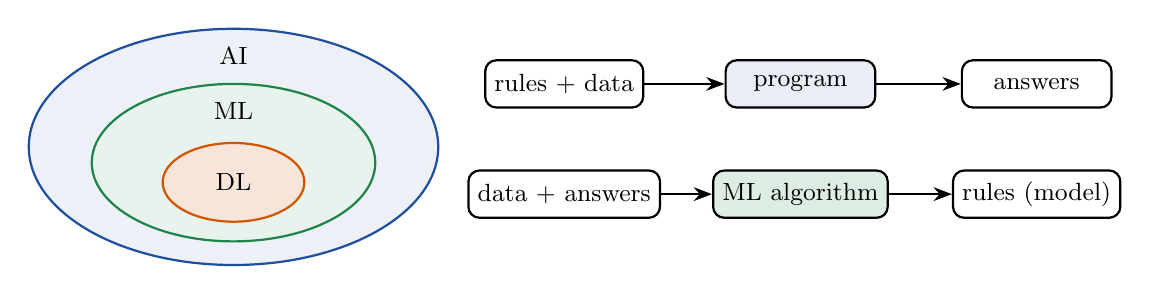
\begin{tikzpicture}[font=\small]
\draw[thick,mlblue,fill=mlblue!8] (0,0) ellipse (2.6 and 1.5); \node at (0,1.15) {AI};
\draw[thick,mlgreen,fill=mlgreen!10] (0,-0.2) ellipse (1.8 and 1.0); \node at (0,0.45) {ML};
\draw[thick,mlorange,fill=mlorange!15] (0,-0.45) ellipse (0.9 and 0.5); \node at (0,-0.45) {DL};
\begin{scope}[xshift=4.2cm,box/.style={draw,rounded corners,thick,minimum width=1.9cm,minimum height=0.6cm}]
\node[box] (r) at (0,0.8) {rules + data}; \node[box,fill=mlblue!10] (p) at (3,0.8) {program}; \node[box] (a) at (6,0.8) {answers};
\draw[-Stealth,thick] (r)--(p); \draw[-Stealth,thick] (p)--(a);
\node[box] (d) at (0,-0.6) {data + answers}; \node[box,fill=mlgreen!15] (m) at (3,-0.6) {ML algorithm}; \node[box] (o) at (6,-0.6) {rules (model)};
\draw[-Stealth,thick] (d)--(m); \draw[-Stealth,thick] (m)--(o);
\end{scope}
\end{tikzpicture}
\end{drawit}

\textbf{Applications:} spam filtering, product recommendation, face recognition, speech assistants, fraud detection, medical diagnosis, self-driving cars, language translation, stock forecasting.

\section{Types of Machine Learning Systems}

ML systems are classified on three bases:
\begin{enumerate}
  \item \textbf{Amount and type of supervision:} supervised, unsupervised, semi-supervised, reinforcement.
  \item \textbf{Can it learn incrementally?} batch (offline) vs.\ online learning.
  \item \textbf{How does it generalise?} instance-based vs.\ model-based learning.
\end{enumerate}

\subsection{By supervision}

\begin{dfn}{Supervised learning}
The training data includes the desired outputs, called \textbf{labels}. The model learns a mapping from inputs to labels. \textbf{Classification} predicts a class (spam/not spam); \textbf{regression} predicts a number (house price).
\end{dfn}
\textbf{Algorithms:} k-NN, linear and logistic regression, SVM, decision trees, random forests, neural networks.

\begin{dfn}{Unsupervised learning}
The training data is \textbf{unlabelled}; the system finds structure (groups, patterns) by itself.
\end{dfn}
\textbf{Tasks:} clustering (K-Means, DBSCAN), dimensionality reduction (PCA), anomaly detection, association rules (Apriori: ``bread $\Rightarrow$ butter'').

\begin{dfn}{Semi-supervised learning}
Learning from a \textbf{small amount of labelled} data plus a \textbf{large amount of unlabelled} data. Example: a photo app clusters faces (unsupervised), you name one face per person, and it labels all photos.
\end{dfn}

\begin{dfn}{Reinforcement learning}
An \textbf{agent} observes the \textbf{environment}, takes \textbf{actions} and receives \textbf{rewards} or penalties. It learns a \textbf{policy} (which action to take in each state) that maximises the total reward over time. Examples: game playing (AlphaGo), robots learning to walk.
\end{dfn}

\begin{drawit}{Reinforcement learning loop}
\centering
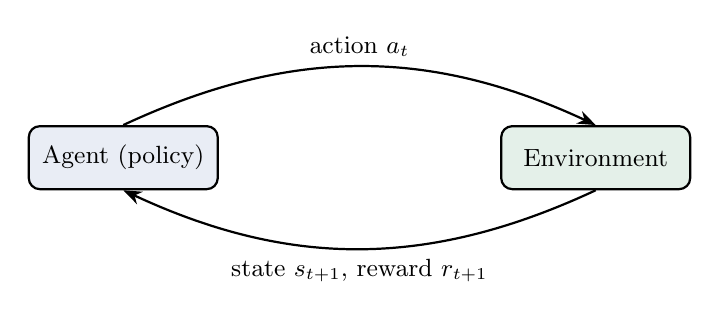
\begin{tikzpicture}[font=\small,box/.style={draw,thick,rounded corners,minimum width=2.4cm,minimum height=0.8cm}]
\node[box,fill=mlblue!10] (a) at (0,0) {Agent (policy)};
\node[box,fill=mlgreen!12] (e) at (6,0) {Environment};
\draw[-Stealth,thick] (a.north) to[bend left=25] node[above]{action $a_t$} (e.north);
\draw[-Stealth,thick] (e.south) to[bend left=25] node[below]{state $s_{t+1}$, reward $r_{t+1}$} (a.south);
\end{tikzpicture}
\end{drawit}

\begin{center}
\small
\begin{tabular}{@{}p{2.0cm}p{3.3cm}p{3.3cm}p{3.3cm}p{3.3cm}@{}}
\toprule
 & \textbf{Supervised} & \textbf{Unsupervised} & \textbf{Semi-supervised} & \textbf{Reinforcement}\\
\midrule
Data & labelled & unlabelled & few labels, many unlabelled & rewards from environment\\
Goal & predict label & find structure & use both & maximise reward\\
Feedback & correct answer & none & partial & delayed reward\\
Example & spam, price & customer groups & photo tagging & games, robots\\
\bottomrule
\end{tabular}
\end{center}

\subsection{Batch vs.\ online learning}
\begin{center}
\small
\begin{tabular}{@{}p{2.8cm}p{6.6cm}p{6.6cm}@{}}
\toprule
 & \textbf{Batch (offline) learning} & \textbf{Online (incremental) learning}\\
\midrule
Training & on all data at once & on small mini-batches, continuously\\
New data & retrain from scratch & learn on the fly\\
Resources & large memory and time & small; suits huge or streaming data\\
Key parameter & --- & \textbf{learning rate}: high = adapts fast but forgets\\
Risk & model becomes stale & bad data quietly degrades it\\
Example & monthly retrained recommender & stock prices, sensor streams\\
\bottomrule
\end{tabular}
\end{center}
\textbf{Out-of-core learning:} online learning used to train on data too large for memory.

\subsection{Instance-based vs.\ model-based learning}
\begin{dfn}{Instance-based learning}
The system \textbf{memorises} the training examples and generalises to a new case by comparing it with stored examples using a \textbf{similarity measure}. Example: k-NN.
\end{dfn}
\begin{dfn}{Model-based learning}
The system builds a \textbf{model} (e.g.\ a line $\hat y=\theta_0+\theta_1x$) from the examples, by choosing parameters that minimise a \textbf{cost function}, and then uses the model to predict.
\end{dfn}
\textbf{Model-based workflow:} study the data $\to$ select a model $\to$ train it (minimise cost) $\to$ apply it to new cases (\textbf{inference}).

\begin{numer}[: least-squares line]
Data $x=(1,2,3,4,5)$ (size), $y=(15,26,29,44,46)$ (price). $\bar x=3$, $\bar y=32$.\\
$S_{xy}=\sum(x-\bar x)(y-\bar y)=34+6+0+12+28=80$, $\ S_{xx}=\sum(x-\bar x)^2=10$.\\
$\theta_1=S_{xy}/S_{xx}=8$, $\ \theta_0=\bar y-\theta_1\bar x=32-24=8$. \textbf{Model} $\hat y=8+8x$; for $x=6$: $\hat y=56$.
\end{numer}

\section{Main Challenges of Machine Learning}
Problems come from either \textbf{bad data} or a \textbf{bad algorithm (model)}.

\begin{enumerate}
  \item \textbf{Insufficient training data:} most algorithms need thousands of examples; ``data matters more than algorithms''.
  \item \textbf{Non-representative data:} training data must represent the new cases. \emph{Sampling noise} (sample too small) and \emph{sampling bias} (flawed sampling method).
  \item \textbf{Poor-quality data:} errors, outliers, missing values. Clean, remove or fill them.
  \item \textbf{Irrelevant features:} garbage in, garbage out. \emph{Feature engineering} = feature selection $+$ feature extraction $+$ creating new features.
  \item \textbf{Overfitting} the training data.
  \item \textbf{Underfitting} the training data.
\end{enumerate}

\begin{dfn}{Overfitting}
\textbf{Overfitting} occurs when the model fits the training data (including its noise) too closely, so it performs well on training data but \textbf{poorly on new data}. Cause: model too complex for the amount and noise of the data.
\end{dfn}
\textbf{Remedies:} simpler model (fewer parameters), more training data, reduce noise, \textbf{regularisation} (constrain the model), cross-validation, early stopping.

\begin{dfn}{Underfitting}
\textbf{Underfitting} occurs when the model is \textbf{too simple} to learn the underlying structure, so it performs poorly even on the training data.
\end{dfn}
\textbf{Remedies:} more powerful model, better features, reduce regularisation.

\begin{drawit}{Underfit, good fit, overfit}
\centering
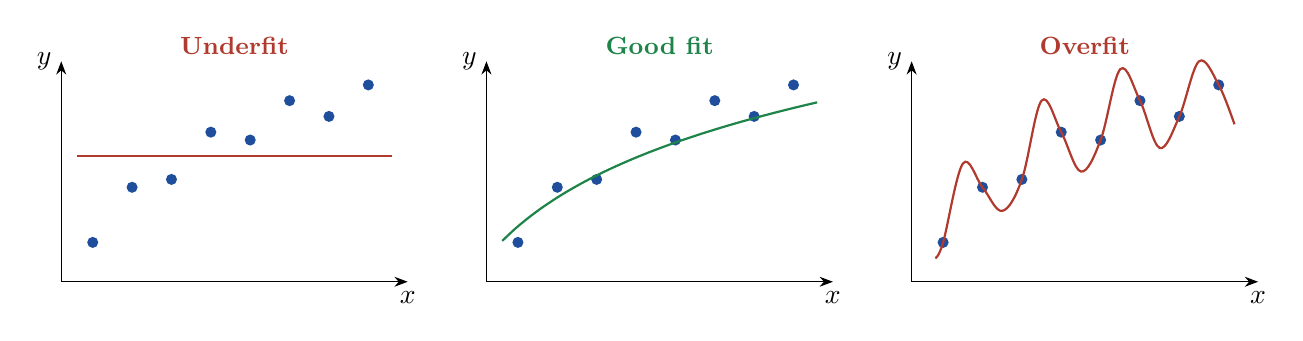
\begin{tikzpicture}
\foreach \k/\t/\c in {0/Underfit/mlred,1/Good fit/mlgreen,2/Overfit/mlred}{
\begin{scope}[xshift=\k*5.4cm]
\draw[-Stealth] (0,0)--(4.4,0) node[below]{$x$}; \draw[-Stealth] (0,0)--(0,2.8) node[left]{$y$};
\foreach \x/\y in {0.4/0.5,0.9/1.2,1.4/1.3,1.9/1.9,2.4/1.8,2.9/2.3,3.4/2.1,3.9/2.5}{\fill[mlblue] (\x,\y) circle(2pt);}
\node[font=\small\bfseries,\c] at (2.2,3.0) {\t};
\end{scope}}
\draw[thick,mlred] (0.2,1.6)--(4.2,1.6);
\draw[thick,mlgreen,domain=0.2:4.2,smooth,xshift=5.4cm] plot (\x,{0.3+1.2*ln(1+\x)});
\draw[thick,mlred,xshift=10.8cm] plot[smooth,tension=0.6] coordinates {(0.3,0.3)(0.4,0.5)(0.65,1.5)(0.9,1.2)(1.15,0.9)(1.4,1.3)(1.65,2.3)(1.9,1.9)(2.15,1.4)(2.4,1.8)(2.65,2.7)(2.9,2.3)(3.15,1.7)(3.4,2.1)(3.65,2.8)(3.9,2.5)(4.1,2.0)};
\end{tikzpicture}
\end{drawit}

\begin{center}
\small
\begin{tabular}{@{}p{2.8cm}p{6.6cm}p{6.6cm}@{}}
\toprule
 & \textbf{Underfitting} & \textbf{Overfitting}\\
\midrule
Model & too simple & too complex\\
Training error & high & very low\\
Test error & high & high\\
Bias / variance & high bias & high variance\\
Fix & more complex model, better features & more data, regularisation, simpler model\\
\bottomrule
\end{tabular}
\end{center}

\section{Testing and Validating}
\begin{itemize}
  \item Split data into \textbf{training set} (usually 80\%) and \textbf{test set} (20\%). The error on new cases is the \textbf{generalisation error}, estimated on the test set.
  \item Training error low but generalisation error high $\Rightarrow$ overfitting.
  \item \textbf{Hyperparameter:} a parameter of the learning algorithm (not of the model), set \emph{before} training, e.g.\ $k$ in k-NN, regularisation strength. \textbf{Parameters} (weights) are learned.
  \item \textbf{Validation set (holdout validation):} part of the training set used to compare models and tune hyperparameters; the test set is used only once at the end.
  \item \textbf{Cross-validation:} rotate the validation part (see Chapter~\ref{n:stat}).
  \item \textbf{No Free Lunch theorem:} no model is best for every problem; you must try several.
\end{itemize}

\begin{imp}
Most asked: Mitchell's definition with a $(T,P,E)$ example; types of ML with a table; overfitting vs.\ underfitting with a diagram; challenges of ML. Always give one real-life example for each type.
\end{imp}

\begin{iq}
\item \twom Define machine learning. Give $T$, $P$, $E$ for a spam filter.
\item \twom Differentiate between AI and ML.
\item \twom What is a hyperparameter? Give an example.
\item \twom What is semi-supervised learning?
\item \fivem Compare supervised and unsupervised learning with examples.
\item \fivem Explain batch and online learning.
\item \fivem Explain instance-based and model-based learning.
\item \fivem What is overfitting? How can it be avoided?
\item \tenm Explain the types of machine learning systems in detail with examples and a diagram.
\item \tenm Discuss the main challenges of machine learning.
\end{iq}

\chapter{Statistical Learning}\label{n:stat}
\studytime{2.5 hours}

\section{Statistical Learning: the Basic Model}

\begin{dfn}{Statistical learning}
\textbf{Statistical learning} is a set of tools for estimating the relationship $f$ between input variables $X=(X_1,\dots,X_p)$ (predictors, features) and an output $Y$ (response):
\[ Y=f(X)+\varepsilon, \]
where $f$ is fixed but unknown and $\varepsilon$ is a random error with mean zero, independent of $X$.
\end{dfn}

\begin{itemize}
  \item \textbf{Why estimate $f$?} (i)~\textbf{Prediction}: $\hat Y=\hat f(X)$ (treat $\hat f$ as a black box). (ii)~\textbf{Inference}: understand \emph{how} $Y$ depends on each $X_j$.
  \item \textbf{Reducible error:} $[f(X)-\hat f(X)]^2$, can be reduced with a better model.
  \item \textbf{Irreducible error:} $\Var(\varepsilon)=\sigma^2$, cannot be removed by any model.
\end{itemize}
\[ \E[(Y-\hat Y)^2]=\underbrace{[f(X)-\hat f(X)]^2}_{\text{reducible}}+\underbrace{\sigma^2}_{\text{irreducible}} \]

\textbf{How to estimate $f$:}
\begin{itemize}
  \item \textbf{Parametric methods:} assume a form (e.g.\ linear), then estimate a few parameters. Simple, but wrong form $\Rightarrow$ poor fit.
  \item \textbf{Non-parametric methods:} no fixed form (e.g.\ k-NN, splines). Flexible, but need much data and may overfit.
\end{itemize}

\section{Supervised vs.\ Unsupervised Learning}
\begin{itemize}
  \item \textbf{Supervised:} for every $x_i$ there is a response $y_i$; fit a model to predict $y$. Regression (quantitative $y$) or classification (qualitative $y$).
  \item \textbf{Unsupervised:} only $x_i$, no $y_i$. Goal: understand relationships between variables or observations, e.g.\ \textbf{cluster analysis}.
  \item \textbf{Semi-supervised:} $y$ known for only some observations.
\end{itemize}

\section{Loss Functions, Training and Test Loss}

\begin{dfn}{Loss function}
A \textbf{loss function} $L(y,\hat y)$ measures the penalty for predicting $\hat y$ when the true value is $y$.
\end{dfn}
\begin{center}
\small
\begin{tabular}{@{}lll@{}}
\toprule
\textbf{Loss} & \textbf{Formula} & \textbf{Used for}\\
\midrule
Squared loss & $(y-\hat y)^2$ & regression (MSE)\\
Absolute loss & $|y-\hat y|$ & regression (MAE), robust to outliers\\
0--1 loss & $\mathbb 1[y\ne\hat y]$ & classification (error rate)\\
Log-loss & $-[y\ln p+(1-y)\ln(1-p)]$ & probabilistic classification\\
\bottomrule
\end{tabular}
\end{center}

\begin{dfn}{Training loss and test loss}
\textbf{Training loss} is the average loss on the data used to fit the model: $\frac1n\sum_{i=1}^nL(y_i,\hat f(x_i))$. \textbf{Test loss} is the average loss on new, unseen data. The test loss measures how well the model \textbf{generalises}.
\end{dfn}

\begin{itemize}
  \item Training loss always falls as model \textbf{flexibility} increases.
  \item Test loss is \textbf{U-shaped}: it falls, reaches a minimum, then rises (overfitting).
  \item A small training loss does \textbf{not} guarantee a small test loss.
\end{itemize}

\begin{drawit}{Training and test loss vs.\ flexibility}
\centering
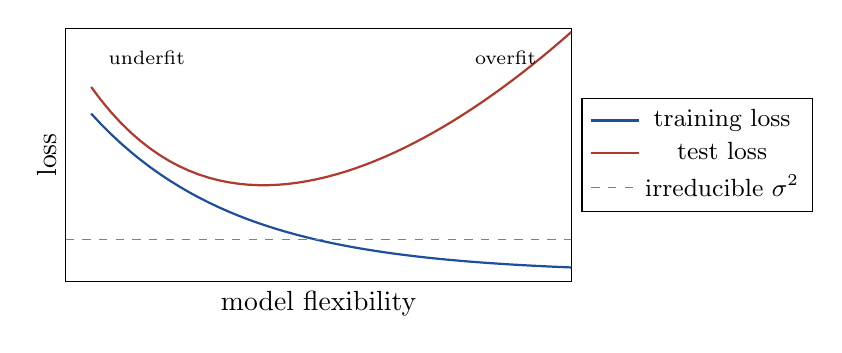
\begin{tikzpicture}
\begin{axis}[width=8cm,height=4.8cm,xlabel={model flexibility},ylabel={loss},ticks=none,xmin=0,xmax=10,ymin=0,ymax=6,legend style={font=\small,at={(1.02,0.5)},anchor=west}]
\addplot[thick,mlblue,domain=0.5:10,samples=50]{4.5*exp(-0.35*x)+0.2}; \addlegendentry{training loss}
\addplot[thick,mlred,domain=0.5:10,samples=50]{4.5*exp(-0.45*x)+0.06*(x-1)^2+1}; \addlegendentry{test loss}
\addplot[dashed,gray,domain=0:10]{1}; \addlegendentry{irreducible $\sigma^2$}
\node[font=\scriptsize] at (axis cs:1.6,5.3) {underfit};
\node[font=\scriptsize] at (axis cs:8.7,5.3) {overfit};
\end{axis}
\end{tikzpicture}
\end{drawit}

\begin{numer}[: computing losses]
$y=(3,5,2)$, $\hat y=(2.5,5,4)$. Errors $=(0.5,0,-2)$.\\
MSE $=\frac{0.25+0+4}{3}=1.417$;\quad RMSE $=\sqrt{1.417}=1.190$;\quad MAE $=\frac{0.5+0+2}{3}=0.833$.
\end{numer}

\section{Risk and Its Estimation}
\begin{dfn}{Risk and empirical risk}
The \textbf{risk} of a model $f$ is its \textbf{expected loss} over the whole population: $\mathcal R(f)=\E[L(Y,f(X))]$. Because the population is unknown, we use the \textbf{empirical risk} (average loss on a sample): $\hat{\mathcal R}(f)=\frac1n\sum_iL(y_i,f(x_i))$.
\end{dfn}

\textbf{Estimating risk (test error):}
\begin{enumerate}
  \item \textbf{Validation-set approach:} split into training and validation parts. Simple, but the estimate varies a lot and uses less data.
  \item \textbf{Leave-one-out CV (LOOCV):} train on $n-1$ points, test on 1, repeat $n$ times. Low bias, but costly.
  \item \textbf{k-fold cross-validation:} split data into $k$ folds; each fold is the validation set once:
  \[ \mathrm{CV}_{(k)}=\frac1k\sum_{i=1}^kE_i \qquad (k=5\text{ or }10). \]
\end{enumerate}

\begin{drawit}{5-fold cross-validation}
\centering
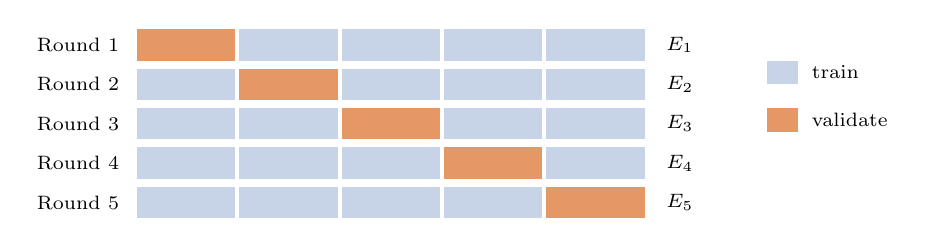
\begin{tikzpicture}[font=\scriptsize]
\foreach \r in {1,...,5}{
  \node[anchor=east] at (-0.1,-\r*0.5) {Round \r};
  \foreach \c in {1,...,5}{
    \ifnum\c=\r \fill[mlorange!60] (\c*1.3-1.3,-\r*0.5-0.2) rectangle ++(1.25,0.4);
    \else \fill[mlblue!25] (\c*1.3-1.3,-\r*0.5-0.2) rectangle ++(1.25,0.4); \fi}
  \node[anchor=west] at (6.6,-\r*0.5) {$E_\r$};}
\fill[mlblue!25] (8,-1) rectangle ++(0.4,0.3); \node[anchor=west] at (8.45,-0.85) {train};
\fill[mlorange!60] (8,-1.6) rectangle ++(0.4,0.3); \node[anchor=west] at (8.45,-1.45) {validate};
\end{tikzpicture}
\end{drawit}

\begin{numer}[: 5-fold CV]
Fold errors $0.20,0.25,0.15,0.22,0.18$. $\ \mathrm{CV}_{(5)}=\frac{1.00}{5}=\mathbf{0.20}$.
\end{numer}

\section{Trade-offs in Statistical Learning}

\subsection{Bias--variance trade-off}
\begin{dfn}{Bias and variance of a model}
\textbf{Bias} is the error from approximating a complex real problem by a simpler model (systematic error). \textbf{Variance} is the amount by which $\hat f$ would change if it were trained on a different training set (sensitivity to data).
\end{dfn}
\[
\E\big[(y_0-\hat f(x_0))^2\big]=\Bias\big[\hat f(x_0)\big]^2+\Var\big[\hat f(x_0)\big]+\sigma^2
\]
\begin{itemize}
  \item More flexible model $\Rightarrow$ bias $\downarrow$, variance $\uparrow$.
  \item Simple model: high bias (underfit). Complex model: high variance (overfit).
  \item The best model balances both, at the minimum of the test-error curve.
\end{itemize}

\begin{drawit}{Bias--variance trade-off; darts board}
\centering
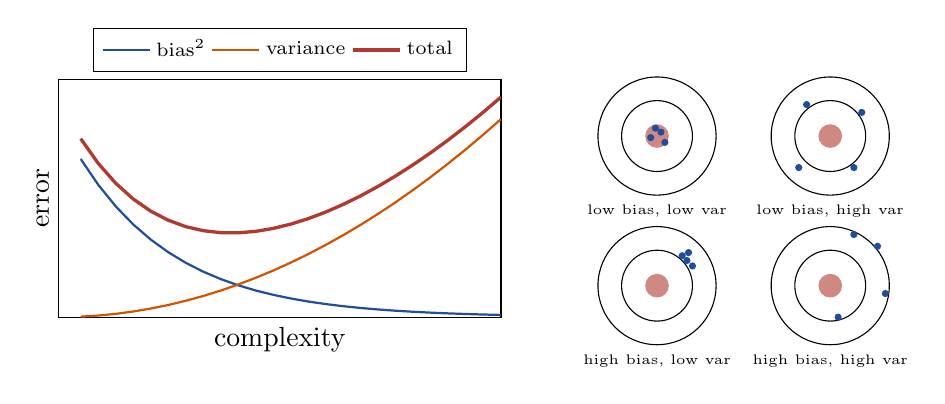
\begin{tikzpicture}
\begin{axis}[width=7.2cm,height=4.6cm,xlabel={complexity},ylabel={error},ticks=none,xmin=0,xmax=10,ymin=0,ymax=6,legend style={font=\scriptsize,at={(0.5,1.03)},anchor=south,legend columns=3}]
\addplot[thick,mlblue,domain=0.5:10]{5*exp(-0.45*x)}; \addlegendentry{bias$^2$}
\addplot[thick,mlorange,domain=0.5:10]{0.05*x^2}; \addlegendentry{variance}
\addplot[very thick,mlred,domain=0.5:10]{5*exp(-0.45*x)+0.05*x^2+0.5}; \addlegendentry{total}
\end{axis}
\begin{scope}[xshift=7.6cm,yshift=0.4cm]
\foreach \i/\bx/\by/\sp/\t in {0/0/1.9/0.12/{low bias, low var},1/2.2/1.9/0.5/{low bias, high var},2/0/0/0.12/{high bias, low var},3/2.2/0/0.5/{high bias, high var}}{
\begin{scope}[shift={(\i*0+\bx,\by)}]
\draw (0,0) circle(0.75); \draw (0,0) circle(0.45); \fill[mlred!60] (0,0) circle(0.15);
\node[font=\tiny,below] at (0,-0.75) {\t};
\end{scope}}
\foreach \x/\y in {0.05/1.95,-0.08/1.88,0.1/1.82,-0.02/2.0}{\fill[mlblue] (\x,\y) circle(1.3pt);}
\foreach \x/\y in {2.6/2.2,1.8/1.5,2.5/1.5,1.9/2.3}{\fill[mlblue] (\x,\y) circle(1.3pt);}
\foreach \x/\y in {0.38/0.32,0.45/0.25,0.32/0.38,0.4/0.42}{\fill[mlblue] (\x,\y) circle(1.3pt);}
\foreach \x/\y in {2.8/0.5,2.3/-0.4,2.9/-0.1,2.5/0.65}{\fill[mlblue] (\x,\y) circle(1.3pt);}
\end{scope}
\end{tikzpicture}
\end{drawit}

\subsection{Other trade-offs}
\begin{itemize}
  \item \textbf{Prediction accuracy vs.\ interpretability:} linear regression and trees are easy to explain; boosting and neural networks are accurate but black boxes.
  \item \textbf{Flexibility vs.\ data size:} flexible models need more data.
  \item \textbf{Parsimony (Occam's razor):} prefer the simplest model that explains the data.
\end{itemize}

\section{Classification Metrics}
\begin{center}
\small
\begin{tabular}{@{}c|cc@{}}
 & \textbf{Predicted +} & \textbf{Predicted $-$}\\ \hline
\textbf{Actual +} & TP & FN\\
\textbf{Actual $-$} & FP & TN\\
\end{tabular}
\end{center}
\[
\text{Accuracy}=\frac{TP+TN}{\text{all}},\quad \text{Precision}=\frac{TP}{TP+FP},\quad \text{Recall}=\frac{TP}{TP+FN},\quad F_1=\frac{2PR}{P+R}.
\]
\begin{itemize}
  \item \textbf{Precision:} of predicted positives, how many are correct. Important when FP is costly (spam folder).
  \item \textbf{Recall (sensitivity):} of actual positives, how many are found. Important when FN is costly (cancer test).
  \item Accuracy misleads on \textbf{imbalanced} data (99\% ``not fraud'' is 99\% accurate yet useless).
\end{itemize}

\begin{numer}[: confusion matrix]
100 e-mails: $TP=40$, $FN=10$, $FP=5$, $TN=45$. Accuracy $=0.85$; Precision $=40/45=0.889$; Recall $=40/50=0.80$; $F_1=\frac{2(0.889)(0.8)}{1.689}=0.842$.
\end{numer}

\section{Sampling Distribution of an Estimator}

\begin{dfn}{Estimator and sampling distribution}
An \textbf{estimator} $\hat\theta$ is a rule (statistic) that computes an estimate of a population parameter $\theta$ from a sample (e.g.\ the sample mean $\bar X$ for $\mu$). The \textbf{sampling distribution} of $\hat\theta$ is the probability distribution of its values over all possible samples of the same size.
\end{dfn}

\begin{itemize}
  \item \textbf{Bias:} $\Bias(\hat\theta)=\E[\hat\theta]-\theta$; unbiased if $0$. $\ \mathrm{MSE}(\hat\theta)=\Var(\hat\theta)+\Bias^2$.
  \item \textbf{Standard error:} standard deviation of the sampling distribution. For the mean: $\mathrm{SE}(\bar X)=\sigma/\sqrt n$.
  \item \textbf{Central Limit Theorem:} for large $n$ ($\ge30$), $\bar X\approx\mathcal N(\mu,\sigma^2/n)$, whatever the population shape.
  \item \textbf{95\% confidence interval:} $\bar x\pm1.96\,s/\sqrt n$.
  \item \textbf{Sample variance} $s^2=\frac{1}{n-1}\sum(x_i-\bar x)^2$ is unbiased; dividing by $n$ is biased (too small).
  \item \textbf{Bootstrap:} estimate SE by resampling the data with replacement many times.
  \item 4 times more data $\Rightarrow$ SE halves.
\end{itemize}

\begin{numer}[: standard error and CI]
$\bar x=70$, $\sigma=10$, $n=25$. $\ \mathrm{SE}=10/\sqrt{25}=2$. 95\% CI $=70\pm1.96(2)=70\pm3.92=(66.08,\,73.92)$.
\end{numer}

\begin{imp}
Most asked: bias--variance trade-off (formula + diagram), training vs.\ test loss (U-curve), k-fold cross-validation, standard error and CLT, precision/recall numerical.
\end{imp}

\begin{iq}
\item \twom What is statistical learning? Write $Y=f(X)+\varepsilon$ and explain.
\item \twom Differentiate reducible and irreducible error.
\item \twom Define risk and empirical risk.
\item \twom What is the standard error of the mean?
\item \fivem Compare parametric and non-parametric methods.
\item \fivem Explain k-fold cross-validation with a diagram.
\item \fivem Explain training loss and test loss with a graph.
\item \fivem State the central limit theorem and its importance.
\item \tenm Explain the bias--variance trade-off with formula and diagram.
\item \tenm Explain the sampling distribution of an estimator, bias, standard error and confidence interval with an example.
\end{iq}

\chapter{Distance-Based Methods, Decision Trees and Naive Bayes}\label{n:knn}
\studytime{2.5 hours}

\section{Distance-Based Methods}
\begin{dfn}{Distance-based learning}
\textbf{Distance-based methods} classify or predict a new instance from the training instances that are \textbf{closest} to it, using a distance (or similarity) measure. Assumption: similar inputs have similar outputs.
\end{dfn}

\begin{center}
\small
\begin{tabular}{@{}lll@{}}
\toprule
\textbf{Measure} & \textbf{Formula} & \textbf{Note}\\
\midrule
Euclidean ($L_2$) & $\sqrt{\sum_i(a_i-b_i)^2}$ & straight-line; most common\\
Manhattan ($L_1$) & $\sum_i|a_i-b_i|$ & city-block distance\\
Minkowski ($L_p$) & $\big(\sum_i|a_i-b_i|^p\big)^{1/p}$ & $p=1$: Manhattan, $p=2$: Euclidean\\
Chebyshev ($L_\infty$) & $\max_i|a_i-b_i|$ & largest single difference\\
Cosine similarity & $\dfrac{\vect a\cdot\vect b}{\|\vect a\|\|\vect b\|}$ & text documents; direction only\\
Hamming & number of positions that differ & categorical / binary data\\
\bottomrule
\end{tabular}
\end{center}

\begin{numer}[: distances]
$\vect a=(1,2)$, $\vect b=(4,6)$. Euclidean $=\sqrt{9+16}=5$; Manhattan $=3+4=7$; Chebyshev $=\max(3,4)=4$.
\end{numer}

\textbf{Feature scaling is essential:} a feature measured in large units (salary in rupees) dominates one in small units (age). Use
\[
\text{min--max: } x'=\frac{x-x_{\min}}{x_{\max}-x_{\min}}\in[0,1],\qquad \text{z-score: } x'=\frac{x-\mu}{\sigma}.
\]

\section{k-Nearest Neighbours (k-NN)}
\begin{dfn}{k-Nearest Neighbours}
\textbf{k-NN} is a supervised, \textbf{instance-based} (lazy) learning algorithm that predicts the class of a new point by the \textbf{majority vote} of its $k$ nearest training points (classification), or by the \textbf{average} of their values (regression).
\end{dfn}

\textbf{Algorithm:}
\begin{enumerate}
  \item Choose $k$ and a distance measure; scale the features.
  \item Compute the distance from the query point to every training point.
  \item Sort the distances and take the $k$ nearest neighbours.
  \item Classification: majority class; regression: mean of their $y$ values.
\end{enumerate}

\begin{itemize}
  \item \textbf{Lazy learner:} no training phase; all work happens at prediction time.
  \item \textbf{Choice of $k$:} small $k$ $\Rightarrow$ noisy, overfits (high variance); large $k$ $\Rightarrow$ too smooth, underfits (high bias). Choose $k$ by cross-validation; use an \textbf{odd} $k$ for two classes.
  \item \textbf{Weighted k-NN:} weight each neighbour by $1/d$ so closer neighbours count more.
\end{itemize}

\begin{numer}[: k-NN classification]
Query $(5,4)$. Training points with distance: $P_4(6,5)$ B $1.414$; $P_5(7,4)$ B $2.0$; $P_6(5,6)$ B $2.0$; $P_7(4,2)$ A $2.236$; $P_3(3,2)$ A $2.828$; $P_2(2,3)$ A $3.162$; $P_1(1,1)$ A $5.0$.\\
$k=3$: B,B,B $\Rightarrow$ \textbf{B}. $\ k=5$: 3 B vs 2 A $\Rightarrow$ \textbf{B}. $\ k=7$: 4 A vs 3 B $\Rightarrow$ \textbf{A} (prediction depends on $k$).
\end{numer}

\begin{drawit}{k-NN with $k=3$}
\centering
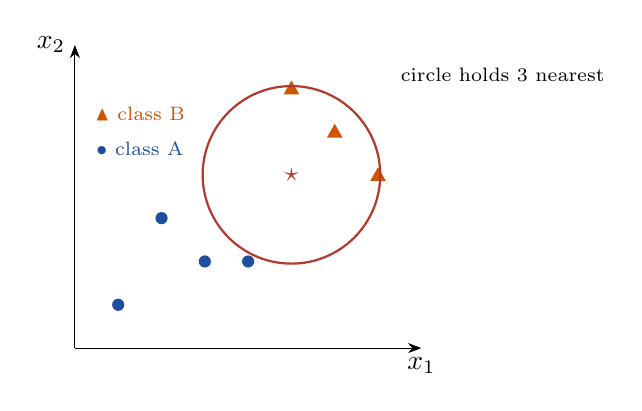
\begin{tikzpicture}[scale=0.55]
\draw[-Stealth] (0,0)--(8,0) node[below]{$x_1$}; \draw[-Stealth] (0,0)--(0,7) node[left]{$x_2$};
\foreach \x/\y in {1/1,2/3,3/2,4/2}{\fill[mlblue] (\x,\y) circle(4pt);}
\foreach \x/\y in {6/5,7/4,5/6}{\fill[mlorange] (\x,\y) ++(0,0.18) -- ++(-0.18,-0.32) -- ++(0.36,0) -- cycle;}
\draw[thick,mlred] (5,4) node{$\star$} circle(2.05);
\node[font=\scriptsize,right] at (7.3,6.3) {circle holds 3 nearest};
\node[font=\scriptsize,mlblue] at (1.5,4.6) {$\bullet$ class A}; \node[font=\scriptsize,mlorange] at (1.5,5.4) {$\blacktriangle$ class B};
\end{tikzpicture}
\end{drawit}

\apa{simple, no training, works for multi-class, naturally non-linear boundaries}{slow prediction on big data, needs scaling, sensitive to irrelevant features and to $k$, suffers from the curse of dimensionality}{recommendation, handwriting recognition, credit rating, medical diagnosis}

\section{Decision Trees}
\begin{dfn}{Decision tree}
A \textbf{decision tree} is a supervised, tree-structured model in which each \textbf{internal node} tests a feature, each \textbf{branch} is an outcome of the test, and each \textbf{leaf node} gives a class label (or value). The tree is built top-down by choosing, at each node, the feature that best separates the classes.
\end{dfn}

\begin{dfn}{Entropy, information gain and Gini index}
\textbf{Entropy} measures the impurity of a set $S$: $H(S)=-\sum_ip_i\log_2p_i$ ($0$ = pure, $1$ = 50/50 for two classes).\\
\textbf{Information gain} is the reduction in entropy after splitting on attribute $A$:
$\ \mathrm{Gain}(S,A)=H(S)-\sum_v\frac{|S_v|}{|S|}H(S_v)$.\\
\textbf{Gini index:} $G=1-\sum_ip_i^2$ (used by CART).
\end{dfn}

\textbf{ID3 algorithm:}
\begin{enumerate}
  \item Compute the entropy of the whole training set.
  \item For each attribute, compute the information gain.
  \item Choose the attribute with the \textbf{highest gain} as the node; create a branch for each value.
  \item Repeat recursively on each branch until all examples in a node have the same class (leaf) or no attributes remain.
\end{enumerate}

\begin{numer}[: information gain (Play-Tennis, 14 days: 9 Yes, 5 No)]
$H(S)=-\frac9{14}\log_2\frac9{14}-\frac5{14}\log_2\frac5{14}=\mathbf{0.940}$.\\
Outlook: Sunny (2Y,3N) $H=0.971$; Overcast (4Y,0N) $H=0$; Rain (3Y,2N) $H=0.971$.\\
$\mathrm{Gain}(\text{Outlook})=0.940-\big[\frac5{14}(0.971)+\frac4{14}(0)+\frac5{14}(0.971)\big]=0.940-0.694=\mathbf{0.246}$.\\
Others: Humidity $0.151$, Wind $0.048$, Temperature $0.029$ $\Rightarrow$ \textbf{Outlook is the root}.
\end{numer}

\begin{numer}[: Gini]
Node with 4 Yes, 6 No: $G=1-(0.4^2+0.6^2)=1-0.52=\mathbf{0.48}$.
\end{numer}

\begin{drawit}{Decision tree for Play-Tennis}
\centering
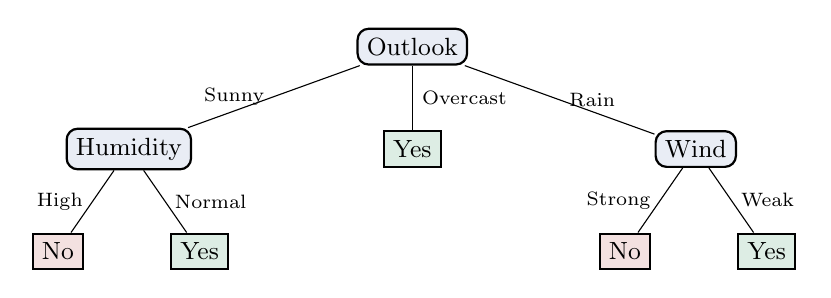
\begin{tikzpicture}[font=\small,level distance=1.3cm,
  level 1/.style={sibling distance=3.6cm},level 2/.style={sibling distance=1.8cm},
  n/.style={draw,thick,rounded corners,fill=mlblue!10},l/.style={draw,thick,fill=mlgreen!15},m/.style={draw,thick,fill=mlred!15}]
\node[n]{Outlook}
  child{node[n]{Humidity} child{node[m]{No} edge from parent node[left,font=\scriptsize]{High}} child{node[l]{Yes} edge from parent node[right,font=\scriptsize]{Normal}} edge from parent node[left,font=\scriptsize]{Sunny}}
  child{node[l]{Yes} edge from parent node[right,font=\scriptsize]{Overcast}}
  child{node[n]{Wind} child{node[m]{No} edge from parent node[left,font=\scriptsize]{Strong}} child{node[l]{Yes} edge from parent node[right,font=\scriptsize]{Weak}} edge from parent node[right,font=\scriptsize]{Rain}};
\end{tikzpicture}
\end{drawit}

\begin{itemize}
  \item \textbf{ID3} uses information gain; \textbf{C4.5} uses gain ratio (handles many-valued attributes, continuous values); \textbf{CART} uses Gini and binary splits (also regression).
  \item \textbf{Overfitting control (pruning):} pre-pruning (max depth, min samples per leaf) or post-pruning (grow fully, then cut weak branches).
\end{itemize}

\apa{easy to understand and draw, no scaling needed, handles numerical and categorical data, gives rules}{overfits easily, unstable (small data change $\Rightarrow$ different tree), biased to many-valued features}{loan approval, medical diagnosis, customer churn, fault diagnosis}

\section{Naive Bayes}
\begin{dfn}{Bayes' theorem}
\[ P(C\mid X)=\frac{P(X\mid C)\,P(C)}{P(X)} \qquad \text{posterior}=\frac{\text{likelihood}\times\text{prior}}{\text{evidence}} \]
\end{dfn}

\begin{dfn}{Naive Bayes classifier}
\textbf{Naive Bayes} is a probabilistic classifier based on Bayes' theorem with the \textbf{naive assumption} that features are \textbf{conditionally independent} given the class:
\[ \hat y=\argmax_c\ P(c)\prod_{j=1}^dP(x_j\mid c). \]
\end{dfn}

\textbf{Steps:} (1) compute priors $P(c)$; (2) compute likelihoods $P(x_j\mid c)$ from frequency tables; (3) multiply for each class; (4) choose the largest.

\begin{dfn}{Laplace smoothing}
If a feature value never occurs with a class, its probability is $0$ and wipes out the whole product. \textbf{Laplace smoothing} adds $\alpha$ (usually 1) to every count:
$\ P(x_j=v\mid c)=\dfrac{\mathrm{count}(v,c)+\alpha}{N_c+\alpha V_j}$, where $V_j$ is the number of values of feature $j$.
\end{dfn}

\begin{numer}[: Bayes' theorem]
$P(\text{spam})=0.3$, $P(\text{offer}\mid\text{spam})=0.6$, $P(\text{offer}\mid\text{ham})=0.1$.\\
$P(\text{spam}\mid\text{offer})=\frac{0.6\times0.3}{0.6\times0.3+0.1\times0.7}=\frac{0.18}{0.25}=\mathbf{0.72}$.
\end{numer}
\begin{numer}[: smoothing]
A value occurs $0$ times among $N_c=10$ examples; the feature has $V=3$ values. Without smoothing $P=0$; with $\alpha=1$: $P=\frac{0+1}{10+3}=\mathbf{0.077}$.
\end{numer}

\apa{very fast, needs little data, works well for text, handles many features and classes}{independence assumption rarely true, zero-frequency problem, probabilities poorly calibrated}{spam filtering, sentiment analysis, document classification, medical diagnosis}

\begin{center}
\small
\begin{tabular}{@{}p{2.6cm}p{4.3cm}p{4.3cm}p{4.3cm}@{}}
\toprule
 & \textbf{k-NN} & \textbf{Decision tree} & \textbf{Naive Bayes}\\
\midrule
Type & instance-based, lazy & model-based (rules) & probabilistic\\
Training & none & builds tree & counts frequencies\\
Prediction speed & slow & fast & very fast\\
Scaling needed & yes & no & no\\
Interpretability & medium & high & medium\\
\bottomrule
\end{tabular}
\end{center}

\begin{imp}
Most asked: k-NN algorithm with a numerical; entropy and information gain numerical (Play-Tennis); Naive Bayes numerical with Laplace smoothing; distance measures.
\end{imp}

\begin{iq}
\item \twom Define Euclidean and Manhattan distance.
\item \twom Why is k-NN called a lazy learner?
\item \twom Define entropy and information gain.
\item \twom Why is Naive Bayes called ``naive''?
\item \fivem Explain the effect of $k$ in k-NN.
\item \fivem Explain Bayes' theorem with an example.
\item \fivem What is pruning? Explain pre- and post-pruning.
\item \tenm Explain the k-NN algorithm with a numerical example; list advantages and disadvantages.
\item \tenm Explain the ID3 algorithm and construct a decision tree using information gain.
\item \tenm Explain the Naive Bayes classifier with Laplace smoothing and a numerical.
\end{iq}

\chapter{Linear Models, GLMs and SVM Basics}\label{n:linear}
\studytime{2.5 hours}

\section{Linear Regression}
\begin{dfn}{Linear regression}
\textbf{Linear regression} is a supervised learning method that models a numerical target as a \textbf{linear combination} of the input features plus an intercept:
$\ \hat y=\theta_0+\theta_1x_1+\dots+\theta_dx_d=\vect\theta^{\!\top}\vect x$.
The parameters are chosen to minimise the \textbf{sum of squared errors} (least squares).
\end{dfn}

\textbf{Cost function:} $J(\vect\theta)=\frac1{2n}\sum_{i=1}^n(\hat y_i-y_i)^2$ (MSE up to a factor).

\textbf{Two ways to find $\vect\theta$:}
\begin{itemize}
  \item \textbf{Closed form (normal equation):} $\vect\theta=(\mathbf X^{\!\top}\mathbf X)^{-1}\mathbf X^{\!\top}\vect y$. For one feature: $\theta_1=S_{xy}/S_{xx}$, $\theta_0=\bar y-\theta_1\bar x$. Exact; slow when $d$ is large ($O(d^3)$).
  \item \textbf{Gradient descent:} iterative; works for huge data.
\end{itemize}

\begin{numer}[: least-squares line and $R^2$]
Hours $x=(1,2,3,4,5)$, marks $y=(35,45,50,65,70)$; $\bar x=3$, $\bar y=53$.\\
$S_{xy}=36+8+0+12+34=90$, $S_{xx}=10$ $\Rightarrow$ $\theta_1=9$, $\theta_0=53-27=26$. \textbf{Model:} $\hat y=26+9x$; $x=6\Rightarrow\hat y=80$.\\
$\hat y=(35,44,53,62,71)$, residuals $(0,1,-3,3,-1)$, SSE $=20$, SST $=\sum(y-\bar y)^2=830$.\\
MSE $=4$, RMSE $=2$, $R^2=1-\frac{20}{830}=\mathbf{0.976}$ (the line explains 97.6\% of the variation).
\end{numer}

\begin{dfn}{Coefficient of determination $R^2$}
$R^2=1-\dfrac{\mathrm{SSE}}{\mathrm{SST}}$: the fraction of the variance of $y$ explained by the model ($0\le R^2\le1$ on training data). \textbf{Adjusted} $R^2=1-(1-R^2)\frac{n-1}{n-p-1}$ penalises extra features.
\end{dfn}

\subsection{Gradient descent}
\begin{dfn}{Gradient descent}
\textbf{Gradient descent} is an iterative optimisation algorithm that minimises a cost function by repeatedly moving the parameters a small step in the direction of the \textbf{negative gradient}:
$\ \theta_j\leftarrow\theta_j-\alpha\,\dfrac{\partial J}{\partial\theta_j}$, where $\alpha$ is the \textbf{learning rate}.
\end{dfn}
For linear regression: $\frac{\partial J}{\partial\theta_0}=\frac1n\sum(\hat y_i-y_i)$, $\ \frac{\partial J}{\partial\theta_1}=\frac1n\sum(\hat y_i-y_i)x_i$.
\begin{itemize}
  \item $\alpha$ too small: very slow; $\alpha$ too large: overshoots and diverges.
  \item \textbf{Batch GD} uses all data per step (smooth, slow); \textbf{Stochastic GD} one example per step (fast, noisy, escapes local minima); \textbf{Mini-batch GD} small batches (best of both, used on GPUs).
  \item Scale features first, otherwise the cost bowl is elongated and GD is slow.
\end{itemize}

\begin{numer}[: one GD step]
Marks data, start $\theta_0=\theta_1=0$, $\alpha=0.01$. All $\hat y=0$.\\
$\frac{\partial J}{\partial\theta_0}=\frac{-(35+45+50+65+70)}{5}=-53$;\ $\frac{\partial J}{\partial\theta_1}=\frac{-(35+90+150+260+350)}{5}=-177$.\\
$\theta_0=0-0.01(-53)=0.53$,\ $\theta_1=0-0.01(-177)=1.77$.
\end{numer}

\begin{drawit}{Gradient descent on a cost curve}
\centering
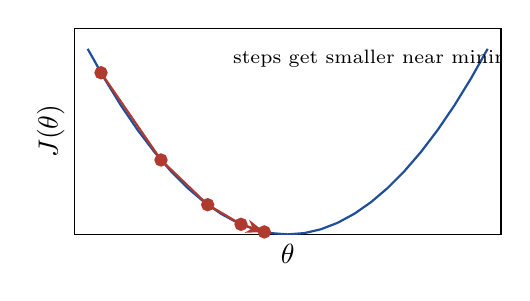
\begin{tikzpicture}
\begin{axis}[width=7cm,height=4.2cm,xlabel={$\theta$},ylabel={$J(\theta)$},ticks=none,xmin=-3.2,xmax=3.2,ymin=0,ymax=10]
\addplot[thick,mlblue,domain=-3:3]{x^2};
\addplot[mlred,mark=*,thick,-Stealth] coordinates {(-2.8,7.84)(-1.9,3.61)(-1.2,1.44)(-0.7,0.49)(-0.35,0.12)};
\node[font=\scriptsize] at (axis cs:1.5,8.5) {steps get smaller near minimum};
\end{axis}
\end{tikzpicture}
\end{drawit}

\subsection{Polynomial regression and regularisation}
\begin{itemize}
  \item \textbf{Polynomial regression:} add powers of features ($x^2,x^3,\dots$) and fit a linear model; high degree $\Rightarrow$ overfitting.
  \item \textbf{Ridge (L2):} $J+\lambda\sum\theta_j^2$, shrinks weights.
  \item \textbf{Lasso (L1):} $J+\lambda\sum|\theta_j|$, sets some weights to zero (feature selection).
  \item \textbf{Elastic Net:} mix of L1 and L2. Larger $\lambda$ $\Rightarrow$ simpler model.
\end{itemize}

\apa{simple, fast, interpretable coefficients, closed-form solution}{assumes linearity, sensitive to outliers and multicollinearity}{price prediction, sales forecasting, trend analysis, risk estimation}

\section{Logistic Regression}
\begin{dfn}{Logistic regression}
\textbf{Logistic regression} is a supervised \textbf{classification} algorithm that estimates the probability that an instance belongs to the positive class by passing a linear combination of the features through the \textbf{sigmoid} function:
$\ p=\sigma(\vect\theta^{\!\top}\vect x)=\dfrac1{1+e^{-\vect\theta^{\!\top}\vect x}}$. Predict 1 if $p\ge0.5$, else 0.
\end{dfn}

\begin{itemize}
  \item Sigmoid maps any $z$ into $(0,1)$; $\sigma(0)=0.5$; $\sigma'(z)=\sigma(z)(1-\sigma(z))$.
  \item \textbf{Odds} $=\frac p{1-p}$; \textbf{log-odds (logit)} $=\ln\frac p{1-p}=\vect\theta^{\!\top}\vect x$ (linear in $x$). One unit increase in $x_j$ multiplies the odds by $e^{\theta_j}$.
  \item \textbf{Decision boundary:} $\vect\theta^{\!\top}\vect x=0$ (a straight line/plane).
  \item \textbf{Cost (log-loss / binary cross-entropy):} $J=-\frac1n\sum\big[y_i\ln p_i+(1-y_i)\ln(1-p_i)\big]$. Convex; no closed form; minimise with GD. Gradient $\frac1n\sum(p_i-y_i)x_{ij}$.
  \item \textbf{Softmax regression} (multinomial): $P(y=k)=\frac{e^{z_k}}{\sum_je^{z_j}}$ for more than two classes.
\end{itemize}

\begin{drawit}{Sigmoid curve}
\centering
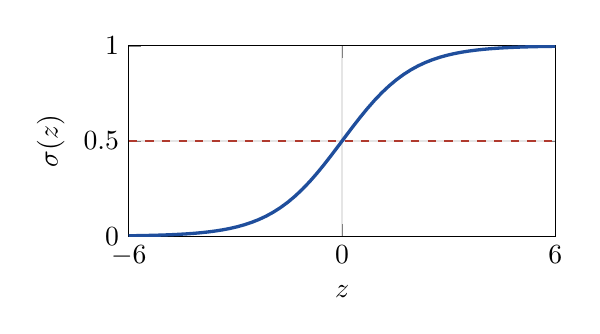
\begin{tikzpicture}
\begin{axis}[width=7cm,height=4cm,xlabel={$z$},ylabel={$\sigma(z)$},xmin=-6,xmax=6,ymin=0,ymax=1,ytick={0,0.5,1},xtick={-6,0,6},grid=major,grid style={gray!20}]
\addplot[very thick,mlblue,domain=-6:6,samples=60]{1/(1+exp(-x))};
\addplot[dashed,mlred] coordinates {(-6,0.5)(6,0.5)};
\end{axis}
\end{tikzpicture}
\end{drawit}

\begin{numer}[: logistic regression]
$\theta_0=-4$, $\theta_1=1$, $x=5$ hours. $z=-4+5=1$, $p=\sigma(1)=\frac1{1+e^{-1}}=\mathbf{0.731}\Rightarrow$ pass.\\
Odds $=0.731/0.269=2.72=e^1$. If $y=1$: log-loss $=-\ln0.731=0.313$.
\end{numer}
\begin{numer}[: softmax]
$z=(2,1,0)$: $e^z=(7.389,2.718,1)$, sum $=11.107$ $\Rightarrow$ $P=(0.665,\,0.245,\,0.090)$; predict class 1.
\end{numer}

\apa{outputs probabilities, simple, interpretable (odds ratios), fast}{linear boundary only, needs feature engineering for complex data, sensitive to outliers}{credit default, disease prediction, spam detection, click-through prediction}

\begin{center}
\small
\begin{tabular}{@{}p{3cm}p{6.6cm}p{6.6cm}@{}}
\toprule
 & \textbf{Linear regression} & \textbf{Logistic regression}\\
\midrule
Task & regression (number) & classification (class/probability)\\
Output & $(-\infty,\infty)$ & $(0,1)$\\
Function & identity & sigmoid\\
Cost & squared error (MSE) & log-loss\\
Solution & closed form or GD & GD only\\
\bottomrule
\end{tabular}
\end{center}

\section{Generalised Linear Models (GLMs)}
\begin{dfn}{Generalised linear model}
A \textbf{GLM} extends linear regression to targets that are not normally distributed. It has three parts: (1) a \textbf{random component}: $y$ follows an exponential-family distribution (normal, Bernoulli, Poisson, \dots); (2) a \textbf{linear predictor} $\eta=\vect\theta^{\!\top}\vect x$; (3) a \textbf{link function} $g$ with $g(\mu)=\eta$, where $\mu=\E[y]$.
\end{dfn}
\begin{center}
\small
\begin{tabular}{@{}llll@{}}
\toprule
\textbf{Model} & \textbf{Distribution of $y$} & \textbf{Link $g(\mu)$} & \textbf{Example}\\
\midrule
Linear regression & Normal & identity $\mu$ & price\\
Logistic regression & Bernoulli & logit $\ln\frac\mu{1-\mu}$ & pass/fail\\
Poisson regression & Poisson & log $\ln\mu$ & number of calls per hour\\
\bottomrule
\end{tabular}
\end{center}
\begin{numer}[: Poisson regression]
$\ln\mu=0.5+0.3x$; $x=2$: $\eta=1.1$, $\mu=e^{1.1}=3.0$ calls. $P(y=0)=e^{-3}=0.0498$. Each extra unit of $x$ multiplies the rate by $e^{0.3}=1.35$.
\end{numer}
GLMs are fitted by \textbf{maximum likelihood}.

\section{Support Vector Machines (basics)}
\begin{dfn}{Support vector machine}
A \textbf{support vector machine (SVM)} is a supervised classifier that finds the \textbf{hyperplane} $\vect w\cdot\vect x+b=0$ separating the two classes with the \textbf{maximum margin}. The training points closest to the hyperplane, which define the margin, are the \textbf{support vectors}.
\end{dfn}
\begin{itemize}
  \item Labels $y_i\in\{-1,+1\}$. Margin width $=\frac2{\|\vect w\|}$.
  \item \textbf{Hard margin:} $\min\frac12\|\vect w\|^2$ s.t.\ $y_i(\vect w\cdot\vect x_i+b)\ge1$ (only for separable data; sensitive to outliers).
  \item \textbf{Soft margin:} allow slack $\xi_i$: $\min\frac12\|\vect w\|^2+C\sum\xi_i$. Large $C$ = few violations, narrow margin; small $C$ = wide margin, more violations.
  \item \textbf{Hinge loss:} $\max(0,\,1-y\,f(\vect x))$.
\end{itemize}

\begin{drawit}{Maximum-margin hyperplane}
\centering
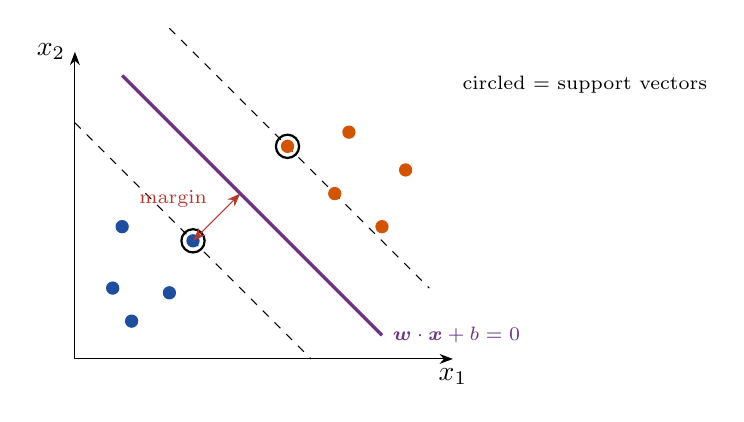
\begin{tikzpicture}[scale=0.6]
\draw[-Stealth] (0,0)--(8,0) node[below]{$x_1$}; \draw[-Stealth] (0,0)--(0,6.5) node[left]{$x_2$};
\draw[very thick,mlpurple] (1,6)--(6.5,0.5) node[right,font=\scriptsize]{$\vect w\cdot\vect x+b=0$};
\draw[dashed] (0,5)--(5,0); \draw[dashed] (2,7)--(7.5,1.5);
\foreach \x/\y in {0.8/1.5,1/2.8,2/1.4,2.5/2.5,1.2/0.8}{\fill[mlblue] (\x,\y) circle(4pt);}
\foreach \x/\y in {5.5/3.5,6.5/2.8,5.8/4.8,7/4,4.5/4.5}{\fill[mlorange] (\x,\y) circle(4pt);}
\draw[thick] (2.5,2.5) circle(7pt); \draw[thick] (4.5,4.5) circle(7pt);
\draw[Stealth-Stealth,mlred] (2.5,2.5)--(3.5,3.5) node[midway,above left,font=\scriptsize]{margin};
\node[font=\scriptsize,right] at (8,5.8) {circled = support vectors};
\end{tikzpicture}
\end{drawit}

\begin{numer}[: margin]
Points $(1,1)$ with $y=-1$ and $(3,3)$ with $y=+1$. Solution $\vect w=(0.5,0.5)$, $b=-2$.\\
Check: $(3,3)\to1.5+1.5-2=+1$; $(1,1)\to0.5+0.5-2=-1$ (both on the margin). Margin $=\frac2{\|\vect w\|}=\frac2{0.707}=\mathbf{2.83}=$ distance between the points. New point $(4,1)$: $2.5-2=0.5>0\Rightarrow+1$.
\end{numer}

\section{Binary Classification}
\begin{itemize}
  \item \textbf{Binary classifier:} two classes (positive/negative), e.g.\ ``digit 5 or not''.
  \item Classifier outputs a \textbf{score}; a \textbf{threshold} turns it into a class. Raising the threshold $\Rightarrow$ precision $\uparrow$, recall $\downarrow$ (\textbf{precision--recall trade-off}).
  \item \textbf{ROC curve:} true positive rate (recall) vs.\ false positive rate ($\frac{FP}{FP+TN}$) for all thresholds. \textbf{AUC} $=1$ perfect, $0.5$ random.
  \item \textbf{Multi-class from binary:} One-vs-Rest ($K$ classifiers) or One-vs-One ($K(K-1)/2$ classifiers).
\end{itemize}

\begin{imp}
Most asked: least-squares line + $R^2$ numerical; gradient descent; logistic regression (sigmoid, odds, log-loss); linear vs.\ logistic table; GLM components; SVM margin and support vectors.
\end{imp}

\begin{iq}
\item \twom Define the learning rate. What if it is too large?
\item \twom What is the sigmoid function? Write its range.
\item \twom What are support vectors?
\item \twom What is a link function?
\item \fivem Compare linear and logistic regression.
\item \fivem Explain batch, stochastic and mini-batch gradient descent.
\item \fivem Explain Ridge and Lasso regularisation.
\item \fivem Explain the ROC curve and the precision--recall trade-off.
\item \tenm Fit a least-squares line to given data, predict a value and compute $R^2$.
\item \tenm Explain logistic regression with its cost function and decision boundary.
\item \tenm Explain generalised linear models with examples.
\end{iq}

\chapter{Ensemble Learning}\label{n:ensemble}
\studytime{2.5 hours}

\begin{dfn}{Ensemble learning}
\textbf{Ensemble learning} combines the predictions of several models (\textbf{base learners}) to obtain a prediction that is more accurate and more stable than that of any single model. A group of predictors is an \textbf{ensemble}; the idea is the ``\textbf{wisdom of the crowd}''.
\end{dfn}
\begin{itemize}
  \item Works best when base learners are \textbf{diverse} (make different, independent errors) and each is better than random guessing (a \textbf{weak learner}).
  \item Diversity comes from: different algorithms, different training subsets, different feature subsets.
  \item Main methods: \textbf{voting}, \textbf{bagging/pasting}, \textbf{random forests}, \textbf{boosting}, \textbf{stacking}.
\end{itemize}

\section{Voting Classifiers}
\begin{dfn}{Voting classifier}
A \textbf{voting classifier} trains several different classifiers on the same data and predicts the class that gets the most votes (\textbf{hard voting}) or the class with the highest \textbf{average predicted probability} (\textbf{soft voting}).
\end{dfn}
\begin{numer}[: majority vote of 3 independent classifiers, each 70\% accurate]
$P(\text{majority correct})=p^3+3p^2(1-p)=0.343+3(0.49)(0.3)=0.343+0.441=\mathbf{0.784}$ (better than 0.70).
\end{numer}
\begin{numer}[: hard vs.\ soft voting]
$P(A)$ from three models $=0.9,\ 0.4,\ 0.4$. Hard vote: A, B, B $\Rightarrow$ \textbf{B}. Soft vote: mean $P(A)=\frac{1.7}3=0.567>0.5\Rightarrow$ \textbf{A}. Soft voting uses confidence and is usually better.
\end{numer}

\section{Bagging and Pasting}
\begin{dfn}{Bagging and pasting}
\textbf{Bagging (Bootstrap Aggregating)} trains the same algorithm on different random subsets of the training set drawn \textbf{with replacement} (bootstrap samples) and aggregates their predictions (vote for classification, average for regression). \textbf{Pasting} is the same but samples \textbf{without replacement}.
\end{dfn}
\textbf{Algorithm:}
\begin{enumerate}
  \item For $b=1,\dots,B$: draw a bootstrap sample of size $n$ from the training data.
  \item Train a model (often a deep decision tree) on it.
  \item Predict by majority vote (classification) or average (regression).
\end{enumerate}
\begin{itemize}
  \item Reduces \textbf{variance} without increasing bias; models train \textbf{in parallel}.
  \item Variance of an average of $B$ models with correlation $\rho$: $\rho\sigma^2+\frac{1-\rho}{B}\sigma^2$. (Example: $\rho=0.5,\sigma^2=1,B=10$: $0.55$ instead of $1$.)
  \item \textbf{Out-of-bag (OOB) evaluation:} each bootstrap sample leaves out about $(1-\frac1n)^n\approx e^{-1}=\mathbf{36.8\%}$ of the instances; they act as a free validation set.
\end{itemize}

\begin{drawit}{Bagging}
\centering
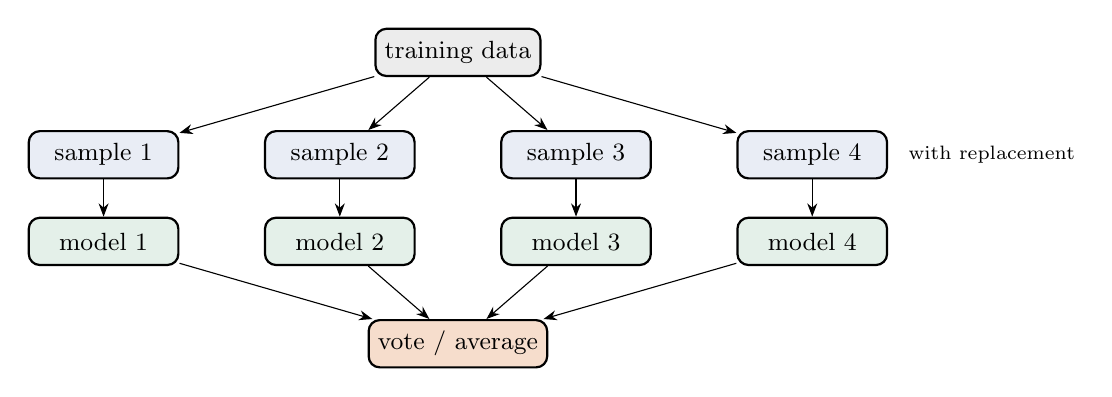
\begin{tikzpicture}[font=\small,b/.style={draw,thick,rounded corners,minimum width=1.9cm,minimum height=0.6cm}]
\node[b,fill=gray!15] (d) at (4.5,2.4) {training data};
\foreach \i/\x in {1/0,2/3,3/6,4/9}{
  \node[b,fill=mlblue!10] (s\i) at (\x,1.1) {sample \i};
  \node[b,fill=mlgreen!12] (m\i) at (\x,0) {model \i};
  \draw[-Stealth] (d)--(s\i); \draw[-Stealth] (s\i)--(m\i);}
\node[b,fill=mlorange!20] (v) at (4.5,-1.3) {vote / average};
\foreach \i in {1,...,4}{\draw[-Stealth] (m\i)--(v);}
\node[font=\scriptsize,right] at (10.1,1.1) {with replacement};
\end{tikzpicture}
\end{drawit}

\section{Random Forests}
\begin{dfn}{Random forest}
A \textbf{random forest} is an ensemble of decision trees trained by bagging, in which each split considers only a \textbf{random subset of features} (typically $\sqrt d$ for classification). The final prediction is the majority vote (or average) of all trees.
\end{dfn}
\begin{itemize}
  \item Two sources of randomness: bootstrap rows + random features $\Rightarrow$ less correlated trees $\Rightarrow$ lower variance than plain bagging.
  \item \textbf{Extra-Trees (extremely randomised trees):} also random split thresholds; faster.
  \item \textbf{Feature importance:} average decrease in impurity caused by each feature over all trees.
  \item Hyperparameters: number of trees, max features, max depth, min samples per leaf.
\end{itemize}
\apa{high accuracy, resists overfitting, handles many features, gives feature importance and OOB score, little tuning}{less interpretable than one tree, slow and large with many trees}{fraud detection, credit scoring, disease prediction, remote sensing, stock analysis}

\section{Boosting}
\begin{dfn}{Boosting}
\textbf{Boosting} trains weak learners \textbf{sequentially}, each new learner focusing on the mistakes of the previous ones, and combines them into a strong learner by a weighted vote.
\end{dfn}

\subsection{AdaBoost (Adaptive Boosting)}
\textbf{Algorithm:}
\begin{enumerate}
  \item Give every training instance equal weight $w_i=\frac1n$.
  \item Train a weak learner $h_t$ (e.g.\ a decision stump); compute weighted error $\varepsilon_t=\sum_{\text{wrong}}w_i$.
  \item Learner weight $\alpha_t=\frac12\ln\frac{1-\varepsilon_t}{\varepsilon_t}$ (more accurate $\Rightarrow$ larger say).
  \item Update $w_i\leftarrow w_i\,e^{-\alpha_ty_ih_t(\vect x_i)}$: wrong instances get \textbf{heavier}; normalise to sum 1.
  \item Repeat; final $H(\vect x)=\operatorname{sign}\big(\sum_t\alpha_th_t(\vect x)\big)$.
\end{enumerate}
\begin{numer}[: one AdaBoost round, 5 instances]
$w=(0.2,\dots,0.2)$; $h_1$ wrong only on instance 4: $\varepsilon_1=0.2$, $\alpha_1=\frac12\ln\frac{0.8}{0.2}=\frac12\ln4=\mathbf{0.693}$.\\
Correct $\times e^{-0.693}=\times0.5\to0.1$; wrong $\times e^{0.693}=\times2\to0.4$. Sum $=0.8$; normalised $w=(0.125,0.125,0.125,\mathbf{0.5},0.125)$.\\
Instance 4 now carries half the weight, so the next learner must get it right.
\end{numer}

\subsection{Gradient boosting}
\begin{itemize}
  \item Each new tree is fitted to the \textbf{residual errors} $r_i=y_i-F_{m-1}(\vect x_i)$ of the current ensemble; $F_m=F_{m-1}+\eta\,h_m$.
  \item $\eta$ (learning rate, \textbf{shrinkage}) small $\Rightarrow$ more trees needed but better generalisation. Use early stopping.
  \item \textbf{XGBoost, LightGBM, CatBoost}: fast, regularised implementations.
\end{itemize}
\begin{numer}[: gradient boosting]
$y=(10,20,30)$. $F_0=\bar y=20$; residuals $(-10,0,10)$. A tree fits them exactly; with $\eta=0.1$: $F_1=20+0.1(-10,0,10)=(19,20,21)$. New residuals $(-9,0,9)$: error shrinks step by step.
\end{numer}

\begin{center}
\small
\begin{tabular}{@{}p{3cm}p{6.6cm}p{6.6cm}@{}}
\toprule
 & \textbf{Bagging} & \textbf{Boosting}\\
\midrule
Training & parallel, independent & sequential, each fixes the last\\
Sampling & bootstrap samples & reweighted (or residual) data\\
Weights of models & equal & by accuracy ($\alpha_t$)\\
Reduces & variance & bias (and variance)\\
Base learner & strong, deep trees & weak learners (stumps)\\
Overfitting & rarely & possible if too many rounds\\
Outliers / noise & robust & sensitive\\
Example & random forest & AdaBoost, gradient boosting\\
\bottomrule
\end{tabular}
\end{center}
\apa{very high accuracy, reduces bias, works with simple learners}{sequential (slow to train), sensitive to noise and outliers, needs careful tuning}{web search ranking, face detection (AdaBoost), Kaggle competitions, credit risk}

\section{Stacking}
\begin{dfn}{Stacking (stacked generalisation)}
\textbf{Stacking} trains several different base models (level 0) and then trains a \textbf{meta-learner} (blender, level 1) that takes the base models' predictions as its inputs and learns how best to combine them.
\end{dfn}
\textbf{Steps:} (1) split training data into two parts (or use cross-validation predictions); (2) train base models on part 1; (3) predict part 2 with them; (4) train the meta-learner on these predictions with the true labels; (5) for new data: base predictions $\to$ meta-learner $\to$ final output.

\begin{drawit}{Stacking}
\centering
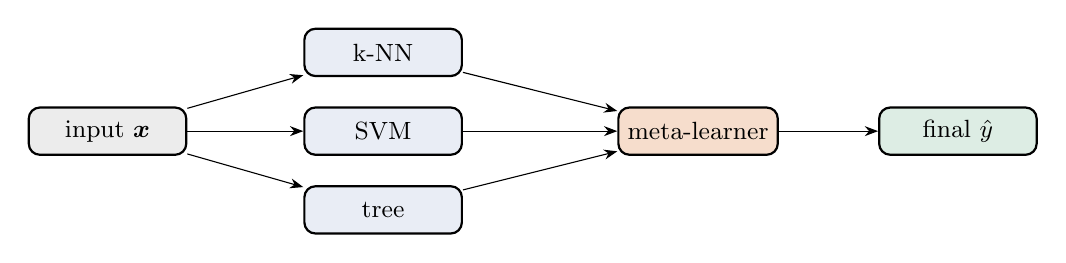
\begin{tikzpicture}[font=\small,b/.style={draw,thick,rounded corners,minimum width=2cm,minimum height=0.6cm}]
\node[b,fill=gray!15] (x) at (0,0) {input $\vect x$};
\node[b,fill=mlblue!10] (a) at (3.5,1) {k-NN}; \node[b,fill=mlblue!10] (b) at (3.5,0) {SVM}; \node[b,fill=mlblue!10] (c) at (3.5,-1) {tree};
\node[b,fill=mlorange!20] (m) at (7.5,0) {meta-learner}; \node[b,fill=mlgreen!15] (y) at (10.8,0) {final $\hat y$};
\foreach \n in {a,b,c}{\draw[-Stealth] (x)--(\n); \draw[-Stealth] (\n)--(m);}
\draw[-Stealth] (m)--(y);
\end{tikzpicture}
\end{drawit}

\begin{center}
\small
\begin{tabular}{@{}lllll@{}}
\toprule
\textbf{Method} & \textbf{Base models} & \textbf{Data per model} & \textbf{Combination} & \textbf{Training}\\
\midrule
Voting & different & same & majority/average & parallel\\
Bagging & same & bootstrap samples & majority/average & parallel\\
Boosting & same (weak) & reweighted & weighted vote & sequential\\
Stacking & different & same (CV) & learned meta-model & two levels\\
\bottomrule
\end{tabular}
\end{center}

\begin{imp}
Most asked: bagging vs.\ boosting table; random forest; AdaBoost algorithm with weights; stacking diagram; hard vs.\ soft voting.
\end{imp}

\begin{iq}
\item \twom Define ensemble learning.
\item \twom Differentiate bagging and pasting.
\item \twom What is out-of-bag evaluation?
\item \twom What is a weak learner?
\item \fivem Explain hard and soft voting with an example.
\item \fivem Explain random forests. Why are they better than a single tree?
\item \fivem Explain stacking with a diagram.
\item \tenm Compare bagging and boosting. Explain the AdaBoost algorithm.
\item \tenm Explain ensemble learning methods: voting, bagging, random forest, boosting and stacking.
\end{iq}

\chapter{Support Vector Machines and Naive Bayes Classifiers}\label{n:svm}
\studytime{2 hours}

\section{Linear SVM Classification}
\begin{dfn}{Large-margin classification}
A \textbf{linear SVM} separates two classes with the hyperplane $\vect w\cdot\vect x+b=0$ that has the \textbf{widest possible margin} (``widest street'') between the classes. Only the \textbf{support vectors} (instances on the edge of the street) determine it; adding points outside the street does not change it.
\end{dfn}
\begin{itemize}
  \item Decision: $\hat y=+1$ if $\vect w\cdot\vect x+b\ge0$, else $-1$. Margin $=2/\|\vect w\|$; maximising it $\equiv$ minimising $\frac12\|\vect w\|^2$.
  \item \textbf{Hard-margin:} all instances off the street; works only if data is linearly separable; very sensitive to outliers.
  \item \textbf{Soft-margin:} balance wide street vs.\ margin violations using slack $\xi_i\ge0$:
  \[\min\ \tfrac12\|\vect w\|^2+C\textstyle\sum_i\xi_i\quad\text{s.t.}\quad y_i(\vect w\cdot\vect x_i+b)\ge1-\xi_i.\]
  \item \textbf{Hyperparameter $C$:} large $C$ $\Rightarrow$ narrow margin, few violations (overfit risk); small $C$ $\Rightarrow$ wide margin, more violations (better generalisation). If the SVM overfits, \textbf{reduce} $C$.
  \item SVMs are sensitive to \textbf{feature scaling}: always standardise.
  \item \textbf{Dual form:} $f(\vect x)=\sum_i\alpha_iy_i(\vect x_i\cdot\vect x)+b$, with $0\le\alpha_i\le C$; $\alpha_i>0$ only for support vectors. The data appears only through dot products $\Rightarrow$ kernel trick.
\end{itemize}

\section{Non-linear SVM Classification}
\begin{itemize}
  \item \textbf{Idea:} map data to a higher-dimensional space $\varphi(\vect x)$ where it becomes linearly separable. Example: 1-D points $x$ not separable $\to$ add $x^2$ $\to$ separable in 2-D.
  \item Adding polynomial features explicitly is slow for high degrees.
\end{itemize}
\begin{dfn}{Kernel trick}
A \textbf{kernel} is a function $K(\vect a,\vect b)=\varphi(\vect a)\cdot\varphi(\vect b)$ that computes the dot product in the transformed space \textbf{without computing the transformation}. The \textbf{kernel trick} replaces every dot product in the SVM by $K$, giving a non-linear classifier at the cost of a linear one.
\end{dfn}
\begin{center}
\small
\begin{tabular}{@{}lll@{}}
\toprule
\textbf{Kernel} & \textbf{Formula} & \textbf{Hyperparameters}\\
\midrule
Linear & $\vect a\cdot\vect b$ & $C$\\
Polynomial & $(\gamma\,\vect a\cdot\vect b+r)^d$ & degree $d$, $r$, $C$\\
Gaussian RBF & $\exp(-\gamma\|\vect a-\vect b\|^2)$ & $\gamma$, $C$\\
Sigmoid & $\tanh(\gamma\,\vect a\cdot\vect b+r)$ & $\gamma$, $r$\\
\bottomrule
\end{tabular}
\end{center}
\begin{itemize}
  \item \textbf{RBF $\gamma$:} large $\gamma$ $\Rightarrow$ narrow bell, wiggly boundary (overfit); small $\gamma$ $\Rightarrow$ smooth boundary (underfit). If overfitting, reduce $\gamma$ (and $C$).
  \item Try linear first (large data, text); then RBF.
\end{itemize}
\begin{numer}[: kernels]
\textbf{Polynomial} $K=(\vect a\cdot\vect b)^2$, $\vect a=(1,2)$, $\vect b=(3,4)$: $\vect a\cdot\vect b=11$, $K=\mathbf{121}$.\\
Check with $\varphi(\vect x)=(x_1^2,\sqrt2x_1x_2,x_2^2)$: $\varphi(\vect a)=(1,2.83,4)$, $\varphi(\vect b)=(9,16.97,16)$, dot $=9+48+64=121$ \checkmark.\\
\textbf{RBF} $\gamma=0.1$, $\vect a=(1,2)$, $\vect b=(2,4)$: $\|\vect a-\vect b\|^2=5$, $K=e^{-0.5}=\mathbf{0.607}$ (similarity).
\end{numer}
\begin{drawit}{Lifting 1-D data with $x^2$}
\centering
\begin{tikzpicture}[scale=0.8]
\draw[-Stealth] (-3.2,0)--(3.2,0) node[right]{$x$};
\foreach \x in {-2.5,-2,2,2.5}{\fill[mlorange] (\x,0) circle(3pt);}
\foreach \x in {-0.8,-0.3,0.4,0.9}{\fill[mlblue] (\x,0) circle(3pt);}
\node[font=\scriptsize] at (0,-0.5) {not linearly separable};
\begin{scope}[xshift=8cm,yshift=-0.5cm]
\draw[-Stealth] (-3.2,0)--(3.2,0) node[right]{$x$}; \draw[-Stealth] (0,0)--(0,3.4) node[left]{$x^2$};
\foreach \x in {-2.5,-2,2,2.5}{\fill[mlorange] (\x,{0.45*\x*\x}) circle(3pt);}
\foreach \x in {-0.8,-0.3,0.4,0.9}{\fill[mlblue] (\x,{0.45*\x*\x}) circle(3pt);}
\draw[thick,mlred,dashed] (-3,1.1)--(3,1.1) node[right,font=\scriptsize]{separating line};
\end{scope}
\end{tikzpicture}
\end{drawit}

\section{SVM Regression (SVR)}
\begin{dfn}{Support vector regression}
\textbf{SVR} reverses the SVM objective: it fits as many instances as possible \textbf{inside} a tube (street) of half-width $\varepsilon$ around the regression function, while keeping the function as flat as possible. Errors inside the tube are ignored ($\varepsilon$-\textbf{insensitive}); only points outside the tube are penalised.
\end{dfn}
\begin{itemize}
  \item $\varepsilon$-insensitive loss: $L_\varepsilon=\max\big(0,\ |y-f(\vect x)|-\varepsilon\big)$.
  \item Problem: $\min\ \frac12\|\vect w\|^2+C\sum(\xi_i+\xi_i^*)$. Support vectors lie on or outside the tube.
  \item Larger $\varepsilon$ $\Rightarrow$ fewer support vectors, flatter model. Kernels (polynomial, RBF) give non-linear SVR.
\end{itemize}
\begin{numer}[: $\varepsilon$-insensitive loss, $\varepsilon=0.5$, $y=10$]
$f=10.3$: $|{-0.3}|<0.5\Rightarrow L=0$. $\quad f=11$: $L=1-0.5=\mathbf{0.5}$. $\quad f=9$: $L=0.5$.
\end{numer}
\apa{effective in high dimensions, memory efficient (uses only support vectors), flexible with kernels, robust (max margin)}{slow on very large data ($O(n^2)$--$O(n^3)$), needs scaling and tuning of $C,\gamma$, no direct probabilities, hard to interpret}{text and image classification, face detection, bioinformatics, handwriting recognition, stock prediction (SVR)}

\section{Naive Bayes Classifiers}
All use $\hat y=\argmax_c\big[\ln P(c)+\sum_j\ln P(x_j\mid c)\big]$ (logs avoid underflow); they differ in how $P(x_j\mid c)$ is modelled.

\begin{dfn}{Gaussian Naive Bayes}
For \textbf{continuous} features, assumes each feature in each class is normally distributed:
$\ P(x_j\mid c)=\dfrac1{\sqrt{2\pi}\sigma_{jc}}\exp\!\Big(-\dfrac{(x_j-\mu_{jc})^2}{2\sigma_{jc}^2}\Big)$, with mean and variance estimated per class. Example: classify fruit by weight and sweetness.
\end{dfn}
\begin{dfn}{Multinomial Naive Bayes}
For \textbf{count} features (word frequencies in text): $\ P(w\mid c)=\dfrac{N_{wc}+\alpha}{N_c+\alpha V}$, where $N_{wc}$ = count of word $w$ in class $c$, $N_c$ = total words in class $c$, $V$ = vocabulary size.
\end{dfn}
\begin{dfn}{Bernoulli Naive Bayes}
For \textbf{binary} features (word present or absent): $P(x_j\mid c)=p_{jc}^{x_j}(1-p_{jc})^{1-x_j}$. Unlike multinomial, it also penalises \textbf{absent} words. Good for short texts.
\end{dfn}

\begin{numer}[: Multinomial NB]
Spam: ``free win'', ``free offer''. Ham: ``meeting today'', ``free meeting''. $V=5$, $N_{\text{spam}}=4$, $N_{\text{ham}}=4$, priors $0.5$. Test: ``free win'' ($\alpha=1$).\\
Spam: $P(\text{free})=\frac{2+1}{9}$, $P(\text{win})=\frac{1+1}9$ $\Rightarrow$ $0.5\times\frac39\times\frac29=0.0370$.\\
Ham: $P(\text{free})=\frac{1+1}{9}$, $P(\text{win})=\frac{0+1}9$ $\Rightarrow$ $0.5\times\frac29\times\frac19=0.0123$.\\
\textbf{Spam} ($P=\frac{0.0370}{0.0493}=0.75$).
\end{numer}

\begin{center}
\small
\begin{tabular}{@{}p{2.6cm}p{4.3cm}p{4.3cm}p{4.3cm}@{}}
\toprule
 & \textbf{Gaussian NB} & \textbf{Multinomial NB} & \textbf{Bernoulli NB}\\
\midrule
Feature type & continuous & counts & binary (0/1)\\
Likelihood & normal density & word frequency & presence/absence\\
Absent features & --- & ignored & penalised\\
Use & sensor, medical data & document classification & short text, spam\\
\bottomrule
\end{tabular}
\end{center}
\apa{fast to train and predict, works with small data and many features, good baseline for text}{independence assumption, zero-frequency problem (needs smoothing), poor probability estimates}{spam filtering, sentiment analysis, news categorisation, real-time prediction}

\begin{center}
\small
\begin{tabular}{@{}p{3.0cm}p{6.6cm}p{6.6cm}@{}}
\toprule
 & \textbf{SVM} & \textbf{Naive Bayes}\\
\midrule
Type & discriminative (boundary) & generative (probabilistic)\\
Speed & slow on large data & very fast\\
Data needed & medium & small\\
Output & class (score) & class probabilities\\
\bottomrule
\end{tabular}
\end{center}

\begin{imp}
Most asked: soft vs.\ hard margin and $C$; kernel trick with polynomial/RBF kernels; effect of $\gamma$; SVR and the $\varepsilon$-tube; three types of Naive Bayes with a table.
\end{imp}

\begin{iq}
\item \twom What is the kernel trick?
\item \twom Write the RBF kernel and explain $\gamma$.
\item \twom What is the $\varepsilon$-insensitive loss?
\item \twom Differentiate multinomial and Bernoulli Naive Bayes.
\item \fivem Explain hard-margin and soft-margin classification.
\item \fivem Explain the role of hyperparameters $C$ and $\gamma$ in SVM.
\item \fivem Explain SVM regression with a diagram.
\item \tenm Explain linear and non-linear SVM classification with the kernel trick.
\item \tenm Explain Gaussian, multinomial and Bernoulli Naive Bayes with an example.
\end{iq}

\chapter{Clustering}\label{n:cluster}
\studytime{2.5 hours}

\begin{dfn}{Clustering}
\textbf{Clustering} is an \textbf{unsupervised} learning task that groups unlabelled instances into \textbf{clusters} so that instances in the same cluster are similar to each other and dissimilar to instances in other clusters.
\end{dfn}
\textbf{Applications:} customer segmentation, data analysis, dimensionality reduction, anomaly (outlier) detection, semi-supervised learning, search engines (similar images), image segmentation.

\textbf{Types:} centroid-based (K-Means), density-based (DBSCAN), distribution-based (Gaussian mixtures), hierarchical (agglomerative).

\section{K-Means}
\begin{dfn}{K-Means}
\textbf{K-Means} partitions $n$ instances into $k$ clusters, each represented by its \textbf{centroid} (mean), by minimising the \textbf{inertia} (within-cluster sum of squared distances):
$\ J=\sum_{j=1}^k\sum_{\vect x_i\in C_j}\|\vect x_i-\vect\mu_j\|^2$.
\end{dfn}
\textbf{Algorithm (Lloyd's):}
\begin{enumerate}
  \item Choose $k$; initialise $k$ centroids (e.g.\ $k$ random instances).
  \item \textbf{Assign} each instance to its nearest centroid.
  \item \textbf{Update} each centroid to the mean of its assigned instances.
  \item Repeat 2--3 until the centroids stop moving.
\end{enumerate}
Inertia never increases, so K-Means always converges, but possibly to a \textbf{local} optimum.

\begin{numer}[: K-Means, $k=2$]
Points $A(2,3)$, $B(5,3)$, $C(5,2)$, $D(1,1)$, $E(4,4)$, $F(4,2)$. Start $\vect\mu_1=C(5,2)$, $\vect\mu_2=F(4,2)$.\\
\textbf{Iter 1:} distances to $(5,2)$ and $(4,2)$: A $3.16/2.24\to2$; B $1.0/1.41\to1$; C $0/1\to1$; D $4.12/3.16\to2$; E $2.24/2.0\to2$; F $1/0\to2$.\\
Clusters $\{B,C\}$, $\{A,D,E,F\}$. New $\vect\mu_1=(5,2.5)$, $\vect\mu_2=(2.75,2.5)$.\\
\textbf{Iter 2:} E ($1.80$ vs $1.95$) and F ($1.12$ vs $1.35$) move to cluster 1. Clusters $\{B,C,E,F\}$, $\{A,D\}$; $\vect\mu_1=(4.5,2.75)$, $\vect\mu_2=(1.5,2)$.\\
\textbf{Iter 3:} no change $\Rightarrow$ \textbf{converged}. Inertia $=3.75+2.5=6.25$.
\end{numer}

\subsection{Choosing $k$ and better initialisation}
\begin{itemize}
  \item \textbf{K-Means++:} choose the first centroid at random, then each next one with probability $\propto D(\vect x)^2$ (distance to nearest chosen centroid) $\Rightarrow$ well spread starting centroids.
  \item \textbf{Multiple runs:} run with different random starts (\texttt{n\_init}) and keep the lowest inertia.
  \item \textbf{Mini-batch K-Means:} uses small batches; much faster on big data.
  \item \textbf{Elbow method:} plot inertia vs.\ $k$; choose the $k$ at the ``elbow'' where the decrease slows.
  \item \textbf{Silhouette coefficient:} $s(i)=\frac{b-a}{\max(a,b)}\in[-1,1]$, $a$ = mean distance to own cluster, $b$ = mean distance to nearest other cluster. $+1$: well placed; $0$: on boundary; $-1$: wrong cluster. Choose $k$ with highest mean silhouette.
\end{itemize}
\begin{numer}[: silhouette]
$a=2$, $b=5$: $s=\frac{5-2}{5}=\mathbf{0.6}$ (well clustered).
\end{numer}

\begin{drawit}{Elbow curve}
\centering
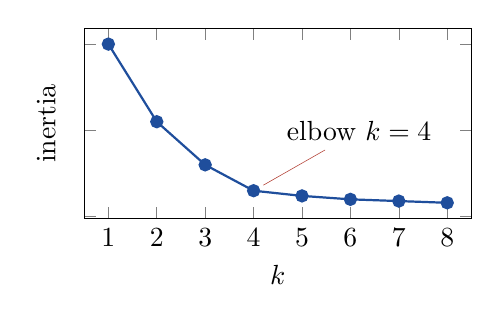
\begin{tikzpicture}
\begin{axis}[width=6.5cm,height=4cm,xlabel={$k$},ylabel={inertia},xtick={1,...,8},yticklabels={},xmin=0.5,xmax=8.5]
\addplot[thick,mlblue,mark=*] coordinates {(1,100)(2,55)(3,30)(4,15)(5,12)(6,10)(7,9)(8,8)};
\node[mlred,font=\scriptsize,pin={[pin edge={mlred}]60:elbow $k=4$}] at (axis cs:4,15) {};
\end{axis}
\end{tikzpicture}
\end{drawit}

\subsection{Limits of K-Means}
\begin{itemize}
  \item $k$ must be specified in advance; result depends on initialisation.
  \item Assumes \textbf{spherical, equal-size, equal-density} clusters; fails on elongated or non-convex shapes (e.g.\ moons, rings).
  \item Sensitive to \textbf{outliers} (the mean is pulled) and to \textbf{feature scale}.
  \item Hard assignment only (no probabilities).
\end{itemize}
\apa{simple, fast, scales to large data, easy to interpret}{needs $k$, local optima, only spherical clusters, sensitive to outliers and scaling}{customer segmentation, image compression/segmentation, document clustering, vector quantisation}

\section{Uses of Clustering}
\begin{itemize}
  \item \textbf{Image segmentation:} partition an image into segments. \textbf{Colour segmentation} clusters the pixel colours (RGB vectors) with K-Means and replaces each pixel by its cluster's mean colour. Example: with $k=8$ colours each pixel needs 3 bits instead of 24 $\Rightarrow$ about $8\times$ smaller.
  \item \textbf{Preprocessing:} replace each instance by its distances to the $k$ centroids (a new, often smaller, feature set) before a classifier. Example: digits data, K-Means with 50 clusters then logistic regression improves accuracy; $k$ tuned with grid search.
  \item \textbf{Semi-supervised learning:} cluster all data and label only the instance nearest each centroid, called a \textbf{representative instance}; then \textbf{propagate} the label to all instances of the cluster. Few labels give high accuracy.
  \item \textbf{Active learning:} the model asks a human to label the instances it is least sure about.
\end{itemize}

\section{DBSCAN}
\begin{dfn}{DBSCAN}
\textbf{DBSCAN} (Density-Based Spatial Clustering of Applications with Noise) defines clusters as continuous regions of \textbf{high density}. With parameters $\varepsilon$ (radius) and \textbf{MinPts}, every instance is a \textbf{core point} (at least MinPts instances, including itself, within distance $\varepsilon$), a \textbf{border point} (not core but within $\varepsilon$ of a core point), or \textbf{noise} (neither).
\end{dfn}
\textbf{Algorithm:}
\begin{enumerate}
  \item For each instance count its $\varepsilon$-neighbours; mark core points.
  \item Connect core points that are within $\varepsilon$ of each other; each connected group is a cluster.
  \item Assign border points to a neighbouring core point's cluster.
  \item Remaining points are noise (anomalies).
\end{enumerate}
\begin{numer}[: DBSCAN, $\varepsilon=1.5$, MinPts $=3$]
$A(1,1)$, $B(1,2)$, $C(2,1)$, $D(2,2)$, $E(3,3)$, $F(8,8)$.\\
A: neighbours B, C, D ($\le1.41$) $\Rightarrow$ 4 $\ge3$: \textbf{core}. Similarly B, C, D are core (D also reaches E at $1.41$).\\
E: only D within $1.5$ $\Rightarrow$ 2 $<3$, but near core D: \textbf{border}. F: alone: \textbf{noise}.\\
Result: one cluster $\{A,B,C,D,E\}$, noise $\{F\}$.
\end{numer}
\begin{drawit}{Core, border and noise points}
\centering
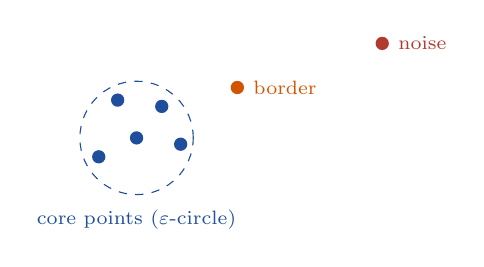
\begin{tikzpicture}[scale=0.8]
\foreach \x/\y in {0/0,0.6/0.3,0.3/0.9,1.0/0.8,1.3/0.2}{\fill[mlblue] (\x,\y) circle(3pt);}
\draw[mlblue,dashed] (0.6,0.3) circle(0.9);
\fill[mlorange] (2.2,1.1) circle(3pt); \fill[mlred] (4.5,1.8) circle(3pt);
\node[font=\scriptsize,mlblue] at (0.6,-1) {core points ($\varepsilon$-circle)};
\node[font=\scriptsize,mlorange,right] at (2.3,1.1) {border};
\node[font=\scriptsize,mlred,right] at (4.6,1.8) {noise};
\end{tikzpicture}
\end{drawit}
\apa{no need to specify $k$, finds clusters of any shape, detects outliers}{hard to choose $\varepsilon$ and MinPts, fails when densities vary, slow in high dimensions, cannot predict new points directly}{anomaly detection, geographic (GPS) data, fraud detection, astronomy}

\begin{center}
\small
\begin{tabular}{@{}p{3cm}p{6.6cm}p{6.6cm}@{}}
\toprule
 & \textbf{K-Means} & \textbf{DBSCAN}\\
\midrule
Basis & distance to centroids & density\\
Number of clusters & must give $k$ & found automatically\\
Cluster shape & spherical & arbitrary\\
Outliers & pulled into clusters & labelled as noise\\
Parameters & $k$ & $\varepsilon$, MinPts\\
\bottomrule
\end{tabular}
\end{center}

\section{Gaussian Mixture Models (GMM)}
\begin{dfn}{Gaussian mixture model}
A \textbf{GMM} is a probabilistic model that assumes the data are generated from a mixture of $k$ Gaussian distributions with unknown parameters:
$\ p(\vect x)=\sum_{j=1}^k\pi_j\,\mathcal N(\vect x\mid\vect\mu_j,\mathbf\Sigma_j)$, $\ \sum\pi_j=1$.
Each cluster is an ellipse with its own mean, covariance (shape/size/orientation) and weight $\pi_j$.
\end{dfn}
\textbf{Expectation--Maximisation (EM) algorithm:}
\begin{enumerate}
  \item Initialise $\pi_j,\vect\mu_j,\mathbf\Sigma_j$ (e.g.\ from K-Means).
  \item \textbf{E-step:} compute the \textbf{responsibility} of each cluster for each instance:
  $\gamma_{ij}=\dfrac{\pi_j\mathcal N(\vect x_i\mid\vect\mu_j,\mathbf\Sigma_j)}{\sum_l\pi_l\mathcal N(\vect x_i\mid\vect\mu_l,\mathbf\Sigma_l)}$.
  \item \textbf{M-step:} update parameters using the responsibilities as weights: $N_j=\sum_i\gamma_{ij}$, $\vect\mu_j=\frac1{N_j}\sum_i\gamma_{ij}\vect x_i$, $\pi_j=N_j/n$, $\mathbf\Sigma_j$ = weighted covariance.
  \item Repeat until the log-likelihood stops increasing.
\end{enumerate}
\begin{numer}[: E-step in 1-D]
$\pi_1=\pi_2=0.5$, $\mu_1=0$, $\mu_2=4$, $\sigma=1$, point $x=1$.\\
$\mathcal N(1\mid0,1)=0.3989e^{-0.5}=0.2420$; $\mathcal N(1\mid4,1)=0.3989e^{-4.5}=0.0044$.\\
$\gamma_1=\frac{0.2420}{0.2420+0.0044}=\mathbf{0.982}$: the point belongs 98\% to cluster 1 (\textbf{soft clustering}).
\end{numer}
\begin{itemize}
  \item EM is like K-Means with \textbf{soft} assignments and elliptical clusters.
  \item \textbf{Choosing $k$:} minimise \textbf{BIC} $=p\ln n-2\ln\hat L$ or \textbf{AIC} $=2p-2\ln\hat L$.
  \item \textbf{Anomaly detection:} instances in low-density regions (below a density threshold) are anomalies.
  \item GMM is a \textbf{generative} model: it can sample new instances.
\end{itemize}
\apa{soft (probabilistic) clustering, elliptical clusters of different sizes, density estimation and anomaly detection, generative}{needs $k$, local optima, slow, many parameters, assumes Gaussian shape}{speaker identification, anomaly detection, image segmentation, finance}

\begin{imp}
Most asked: K-Means algorithm with numerical; limits of K-Means; elbow and silhouette; DBSCAN core/border/noise; K-Means vs.\ DBSCAN; GMM with EM; image segmentation and semi-supervised learning using clustering.
\end{imp}

\begin{iq}
\item \twom Define clustering. Give two applications.
\item \twom What is inertia?
\item \twom Define core point, border point and noise in DBSCAN.
\item \twom What is a responsibility in GMM?
\item \fivem Explain the elbow method and silhouette score.
\item \fivem Explain the limits of K-Means.
\item \fivem How is clustering used for image segmentation and preprocessing?
\item \fivem Explain semi-supervised learning using clustering.
\item \tenm Explain K-Means with an example and its limitations.
\item \tenm Explain DBSCAN and compare it with K-Means.
\item \tenm Explain Gaussian mixture models and the EM algorithm.
\end{iq}

\chapter{Dimensionality Reduction}\label{n:dimred}
\studytime{2 hours}

\begin{dfn}{Dimensionality reduction}
\textbf{Dimensionality reduction} is the process of reducing the number of features (dimensions) of a dataset while keeping as much of the important information as possible.
\end{dfn}
\textbf{Why:} speed up training, remove noise and redundant features, avoid the curse of dimensionality, compress data, visualise data in 2-D or 3-D (\textbf{data visualisation}). \textbf{Cost:} some information is lost; pipelines become more complex.

\section{The Curse of Dimensionality}
\begin{dfn}{Curse of dimensionality}
The \textbf{curse of dimensionality} refers to the problems that arise when data has very many features: the space becomes so large that data is \textbf{sparse}, distances between points become large and similar, and the amount of data needed to generalise grows \textbf{exponentially} with the number of dimensions.
\end{dfn}
\begin{itemize}
  \item In a unit square, a random point is near the border (within 0.001) with probability $0.4\%$; in 10\,000 dimensions $>99.999999\%$. In general $P=1-(1-2\delta)^d$.
  \item Average distance between two random points: $0.52$ in 2-D, $0.66$ in 3-D, about $408.25$ in 1\,000\,000-D $\Rightarrow$ new instances are far from training instances.
  \item To cover a space with $b$ bins per feature you need $b^d$ cells (e.g.\ $10^{100}$ for 100 features).
  \item Effect: high risk of \textbf{overfitting}; distance-based methods (k-NN, K-Means) suffer most.
  \item Remedy: more data (impractical: exponential) or \textbf{reduce dimensions}.
\end{itemize}
\begin{numer}[: near the border]
$\delta=0.001$. $d=2$: $1-0.998^2=0.004$ (0.4\%). $\ d=1000$: $1-0.998^{1000}=1-e^{-2}=\mathbf{0.865}$ (86\%).
\end{numer}

\section{Main Approaches}
\begin{dfn}{Projection}
In most real problems the training instances lie close to a much \textbf{lower-dimensional subspace}. \textbf{Projection} drops perpendicular onto that subspace (e.g.\ 3-D points near a plane are projected to 2-D). PCA is a projection method.
\end{dfn}
\begin{dfn}{Manifold learning}
A $d$-dimensional \textbf{manifold} is a shape that locally looks like a $d$-dimensional plane but is bent or twisted in a higher-dimensional space (e.g.\ the \textbf{Swiss roll}: 2-D manifold in 3-D). \textbf{Manifold learning} models this shape and \textbf{unrolls} it; projection would squash its layers together. Examples: LLE, Isomap, t-SNE.
\end{dfn}
\begin{itemize}
  \item \textbf{Manifold hypothesis:} most real high-dimensional data lie close to a much lower-dimensional manifold.
  \item \textbf{Feature selection} keeps a subset of original features; \textbf{feature extraction} creates new combined features (PCA).
  \item Linear methods: PCA, LDA. Non-linear: Kernel PCA, LLE, t-SNE, autoencoders.
\end{itemize}
\begin{drawit}{Projection vs.\ manifold (Swiss roll)}
\centering
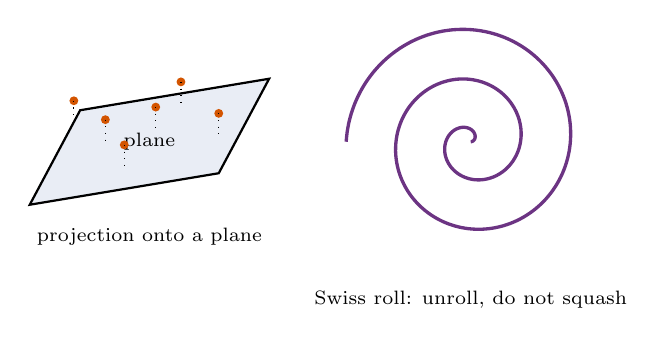
\begin{tikzpicture}[scale=0.8]
\draw[thick,fill=mlblue!10] (0,0)--(3,0.5)--(3.8,2)--(0.8,1.5)--cycle; \node[font=\scriptsize] at (1.9,1) {plane};
\foreach \x/\y in {0.7/1.3,1.5/0.6,2.4/1.6,3/1.1,1.2/1.0,2.0/1.2}{\fill[mlorange] (\x,\y+0.35) circle(2pt); \draw[dotted] (\x,\y+0.35)--(\x,\y);}
\node[font=\scriptsize] at (1.9,-0.5) {projection onto a plane};
\begin{scope}[xshift=7cm,yshift=1cm]
\draw[very thick,mlpurple,domain=0:900,samples=200,smooth] plot ({0.0022*\x*cos(\x)},{0.0022*\x*sin(\x)});
\node[font=\scriptsize] at (0,-2.5) {Swiss roll: unroll, do not squash};
\end{scope}
\end{tikzpicture}
\end{drawit}

\section{Principal Component Analysis (PCA)}
\begin{dfn}{PCA}
\textbf{Principal Component Analysis} is an unsupervised, linear dimensionality-reduction technique that finds new orthogonal axes, the \textbf{principal components}, ordered so that the first captures the \textbf{maximum variance} of the data, the second the maximum remaining variance, and so on. The data is then projected onto the first $m$ components.
\end{dfn}
\begin{itemize}
  \item \textbf{Preserving variance:} the axis that keeps maximum variance also minimises the mean squared distance between original points and their projections (least information lost).
  \item Components are the \textbf{eigenvectors} of the covariance matrix; their \textbf{eigenvalues} are the variances along them.
  \item PCA assumes data is \textbf{centred}; scale features first if units differ.
\end{itemize}
\textbf{Algorithm:}
\begin{enumerate}
  \item Standardise / centre the data: $\tilde{\mathbf X}=\mathbf X-\bar{\mathbf x}$.
  \item Compute the covariance matrix $\mathbf C=\frac1{n-1}\tilde{\mathbf X}^{\!\top}\tilde{\mathbf X}$.
  \item Find eigenvalues and eigenvectors: $\mathbf C\vect w=\lambda\vect w$; sort by $\lambda$ (descending).
  \item Choose $m$ components (e.g.\ 95\% explained variance).
  \item Project: $\mathbf Z=\tilde{\mathbf X}\mathbf W_m$.
\end{enumerate}
In practice PCA is computed with \textbf{SVD}: $\tilde{\mathbf X}=\mathbf U\mathbf S\mathbf V^{\!\top}$; rows of $\mathbf V^{\!\top}$ are the components, $\lambda_j=s_j^2/(n-1)$.

\begin{numer}[: PCA by hand]
Points $(1,1),(2,3),(3,2),(4,5),(5,4)$. Means $\bar x=\bar y=3$; centred: $(-2,-2),(-1,0),(0,-1),(1,2),(2,1)$.\\
$s_{xx}=\frac{10}4=2.5$, $s_{yy}=2.5$, $s_{xy}=\frac{4+0+0+2+2}4=2$ $\Rightarrow$ $\mathbf C=\left[\begin{smallmatrix}2.5&2\\2&2.5\end{smallmatrix}\right]$.\\
$\det(\mathbf C-\lambda\mathbf I)=(2.5-\lambda)^2-4=0\Rightarrow\lambda_1=4.5$, $\lambda_2=0.5$.\\
$\vect w_1=(0.707,0.707)$, $\vect w_2=(0.707,-0.707)$. Explained variance: PC1 $\frac{4.5}{5}=\mathbf{90\%}$, PC2 $10\%$.\\
Project A: $z_1=\frac{-2-2}{\sqrt2}=-2.83$. Keeping only PC1 reduces 2-D to 1-D while keeping 90\% of the variance.
\end{numer}

\begin{drawit}{Principal components of 2-D data}
\centering
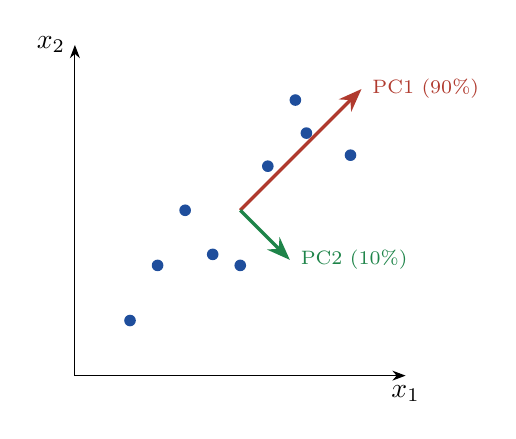
\begin{tikzpicture}[scale=0.7]
\draw[-Stealth] (0,0)--(6,0) node[below]{$x_1$}; \draw[-Stealth] (0,0)--(0,6) node[left]{$x_2$};
\foreach \x/\y in {1/1,2/3,3/2,4/5,5/4,1.5/2,3.5/3.8,2.5/2.2,4.2/4.4}{\fill[mlblue] (\x,\y) circle(3pt);}
\draw[very thick,mlred,-Stealth] (3,3)--(5.2,5.2) node[right,font=\scriptsize]{PC1 (90\%)};
\draw[very thick,mlgreen,-Stealth] (3,3)--(3.9,2.1) node[right,font=\scriptsize]{PC2 (10\%)};
\end{tikzpicture}
\end{drawit}

\begin{itemize}
  \item \textbf{Explained variance ratio} $=\lambda_j/\sum\lambda_i$. Choose $m$ so cumulative ratio $\ge95\%$, or look for the elbow of the \textbf{scree plot}. (MNIST: 784 $\to$ 154 dims keeps 95\%.)
  \item \textbf{Reconstruction:} $\hat{\mathbf X}=\mathbf Z\mathbf W_m^{\!\top}+\bar{\mathbf x}$; reconstruction error $=$ sum of discarded eigenvalues (compression).
  \item \textbf{Randomized PCA} (fast approximation), \textbf{Incremental PCA} (mini-batches, large data), \textbf{Kernel PCA} (non-linear via kernel trick).
\end{itemize}
\apa{reduces dimensions and noise, speeds up learning, removes correlation, helps visualisation, unsupervised}{components hard to interpret, linear only, loses some information, sensitive to scaling and outliers}{image compression, face recognition (eigenfaces), visualisation, gene data, preprocessing for ML}

\begin{center}
\small
\begin{tabular}{@{}p{3cm}p{6.6cm}p{6.6cm}@{}}
\toprule
 & \textbf{Feature selection} & \textbf{Feature extraction (PCA)}\\
\midrule
Output & subset of original features & new features (combinations)\\
Interpretability & high & low\\
Example & drop irrelevant columns & PCA, LDA\\
\bottomrule
\end{tabular}
\end{center}

\begin{imp}
Most asked: curse of dimensionality; projection vs.\ manifold learning; PCA steps with numerical (covariance, eigenvalues, explained variance); choosing number of components.
\end{imp}

\begin{iq}
\item \twom Define dimensionality reduction. Give two reasons for using it.
\item \twom What is the curse of dimensionality?
\item \twom What is a manifold?
\item \twom What is the explained variance ratio?
\item \fivem Explain projection and manifold learning.
\item \fivem How do you choose the number of principal components?
\item \fivem Compare feature selection and feature extraction.
\item \tenm Explain PCA with its algorithm and a numerical example.
\item \tenm Explain the curse of dimensionality and the main approaches to dimensionality reduction.
\end{iq}

\chapter{Artificial Neural Networks with Keras}\label{n:ann}
\studytime{2.5 hours}

\section{From Biological to Artificial Neurons}
\begin{dfn}{Artificial neural network (ANN)}
An \textbf{artificial neural network} is a machine-learning model inspired by the network of biological neurons in the brain. It consists of layers of simple connected units (\textbf{artificial neurons}); each connection has a \textbf{weight} that is learned from data. ANNs are the core of \textbf{deep learning}.
\end{dfn}
\begin{center}
\small
\begin{tabular}{@{}ll@{}}
\toprule
\textbf{Biological neuron} & \textbf{Artificial neuron}\\
\midrule
dendrites (receive signals) & inputs $x_j$\\
synapse strength & weights $w_j$\\
cell body (sums signals) & weighted sum $z=\vect w\cdot\vect x+b$\\
axon fires if above threshold & activation $a=\varphi(z)$\\
\bottomrule
\end{tabular}
\end{center}
\textbf{Why now:} huge data, powerful GPUs, better algorithms (ReLU, Adam, dropout), better initialisation.

\begin{drawit}{Artificial neuron}
\centering
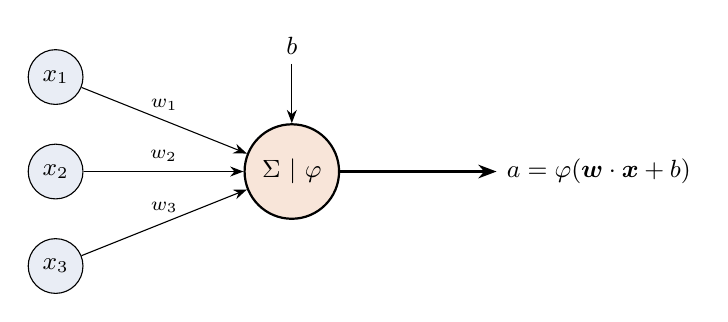
\begin{tikzpicture}[font=\small]
\foreach \i/\y in {1/1.2,2/0,3/-1.2}{\node[draw,circle,fill=mlblue!10] (x\i) at (0,\y) {$x_\i$};}
\node[draw,circle,thick,fill=mlorange!15,minimum size=1.2cm] (s) at (3,0) {$\Sigma\ |\ \varphi$};
\foreach \i in {1,2,3}{\draw[-Stealth] (x\i)--(s) node[midway,above,font=\scriptsize]{$w_\i$};}
\node (b) at (3,1.6) {$b$}; \draw[-Stealth] (b)--(s);
\draw[-Stealth,thick] (s)--(5.6,0) node[right]{$a=\varphi(\vect w\cdot\vect x+b)$};
\end{tikzpicture}
\end{drawit}

\section{The Perceptron}
\begin{dfn}{Perceptron (Rosenblatt, 1957)}
The \textbf{perceptron} is the simplest ANN: a single layer of \textbf{threshold logic units (TLUs)}. Each TLU computes $z=\vect w\cdot\vect x+b$ and outputs a \textbf{step function}: $\hat y=1$ if $z>0$, else $0$. It is a linear binary classifier.
\end{dfn}
\textbf{Perceptron learning rule:} for each training instance, $\ w_j\leftarrow w_j+\eta(y-\hat y)x_j$, $\ b\leftarrow b+\eta(y-\hat y)$. Weights change only on mistakes.
\textbf{Perceptron convergence theorem:} if the data is linearly separable, the rule converges to a solution.

\begin{numer}[: perceptron learns AND ($\eta=1$, start $\vect w=(0,0)$, $b=0$)]
Epoch 1: $(1,1)$ predicted 0, $y=1$ $\Rightarrow$ $\vect w=(1,1)$, $b=1$.\\
Continuing, after epoch 5: $\vect w=(2,1)$, $b=-2$; epoch 6 makes no mistakes.\\
Check: $(1,1)\to1>0\Rightarrow1$; $(1,0)\to0\Rightarrow0$; $(0,1)\to-1\Rightarrow0$; $(0,0)\to-2\Rightarrow0$ \checkmark. Boundary $2x_1+x_2=2$.
\end{numer}

\begin{itemize}
  \item \textbf{XOR problem} (Minsky \& Papert, 1969): XOR is not linearly separable, so a single perceptron cannot learn it. Solution: \textbf{stack} perceptrons $\Rightarrow$ multilayer perceptron. E.g.\ XOR $=$ AND(OR, NAND).
\end{itemize}

\section{Multilayer Perceptron (MLP) and Backpropagation}
\begin{dfn}{Multilayer perceptron}
An \textbf{MLP} consists of an \textbf{input layer}, one or more \textbf{hidden layers} of neurons, and an \textbf{output layer}; every neuron is connected to all neurons of the next layer (\textbf{dense / fully connected}). Signals flow only forward (\textbf{feedforward network}). An ANN with many hidden layers is a \textbf{deep neural network (DNN)}.
\end{dfn}
\begin{drawit}{MLP with one hidden layer}
\centering
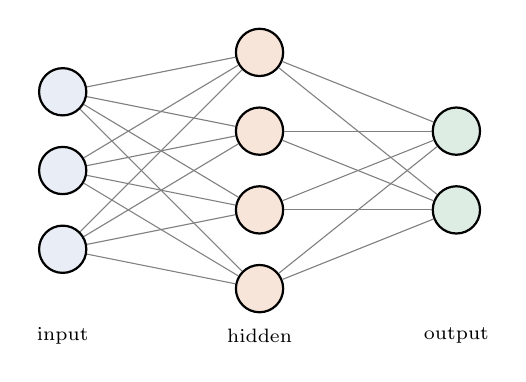
\begin{tikzpicture}[n/.style={circle,draw,thick,minimum size=0.6cm}]
\foreach \i in {1,2,3}{\node[n,fill=mlblue!10] (i\i) at (0,1.5-\i) {};}
\foreach \i in {1,...,4}{\node[n,fill=mlorange!15] (h\i) at (2.5,2-\i) {};}
\foreach \i in {1,2}{\node[n,fill=mlgreen!15] (o\i) at (5,1-\i) {};}
\foreach \a in {1,2,3}{\foreach \b in {1,...,4}{\draw[gray] (i\a)--(h\b);}}
\foreach \a in {1,...,4}{\foreach \b in {1,2}{\draw[gray] (h\a)--(o\b);}}
\node[font=\scriptsize] at (0,-2.6) {input}; \node[font=\scriptsize] at (2.5,-2.6) {hidden}; \node[font=\scriptsize] at (5,-2.6) {output};
\end{tikzpicture}
\end{drawit}

\begin{numer}[: forward pass of a 2--2--1 network (sigmoid)]
$\vect x=(1,0.5)$; hidden: $z_1=0.4(1)-0.6(0.5)+0.1=0.2$, $a_1=\sigma(0.2)=0.5498$; $z_2=0.7(1)+0.2(0.5)-0.2=0.6$, $a_2=0.6457$.\\
Output: $z=0.5(0.5498)-0.3(0.6457)+0.05=0.1312$, $\hat y=\sigma(0.1312)=\mathbf{0.533}$. Parameters $=(2\cdot2+2)+(2+1)=9$.
\end{numer}
\textbf{Parameters of a dense layer} $=n_{\text{in}}n_{\text{out}}+n_{\text{out}}$. MLP 784--300--100--10: $235\,500+30\,100+1\,010=\mathbf{266\,610}$.

\begin{dfn}{Backpropagation}
\textbf{Backpropagation} is the algorithm used to train MLPs. For each mini-batch it makes a \textbf{forward pass} (compute outputs and loss), then a \textbf{backward pass} that uses the \textbf{chain rule} to compute the gradient of the loss with respect to every weight, layer by layer from output to input, and finally a \textbf{gradient descent step} to update the weights.
\end{dfn}
\textbf{Steps:}
\begin{enumerate}
  \item Initialise weights randomly (not zero: symmetry breaking).
  \item Forward pass: compute every layer's output and the loss.
  \item Output error: $\delta^{(L)}=\frac{\partial J}{\partial a^{(L)}}\odot\varphi'(z^{(L)})$.
  \item Propagate back: $\delta^{(l)}=(\mathbf W^{(l+1)\top}\delta^{(l+1)})\odot\varphi'(z^{(l)})$.
  \item Gradients: $\frac{\partial J}{\partial\mathbf W^{(l)}}=\delta^{(l)}a^{(l-1)\top}$; update $\mathbf W\leftarrow\mathbf W-\eta\frac{\partial J}{\partial\mathbf W}$.
  \item Repeat for all mini-batches; one pass over the training set is an \textbf{epoch}.
\end{enumerate}
Step function has zero gradient, so MLPs use smooth activations.

\section{Activation Functions}
\begin{center}
\small
\begin{tabular}{@{}llll@{}}
\toprule
\textbf{Function} & \textbf{Formula} & \textbf{Range} & \textbf{Note}\\
\midrule
Sigmoid & $\frac1{1+e^{-z}}$ & $(0,1)$ & binary output; vanishing gradient\\
Tanh & $\frac{e^z-e^{-z}}{e^z+e^{-z}}$ & $(-1,1)$ & zero-centred\\
ReLU & $\max(0,z)$ & $[0,\infty)$ & default for hidden layers; fast; ``dying ReLU''\\
Leaky ReLU & $\max(\alpha z,z)$ & $(-\infty,\infty)$ & fixes dying ReLU\\
Softmax & $\frac{e^{z_k}}{\sum_je^{z_j}}$ & $(0,1)$, sum 1 & multi-class output\\
\bottomrule
\end{tabular}
\end{center}
\textbf{Why non-linear?} Without non-linear activations, many layers collapse into a single linear transformation and cannot learn complex patterns.

\begin{center}
\small
\begin{tabular}{@{}p{3.0cm}p{3.2cm}p{3.2cm}p{5.5cm}@{}}
\toprule
\textbf{Task} & \textbf{Output neurons} & \textbf{Output activation} & \textbf{Loss}\\
\midrule
Regression & 1 per value & none (linear) & MSE (or MAE, Huber)\\
Binary classification & 1 & sigmoid & binary cross-entropy\\
Multi-label & 1 per label & sigmoid & binary cross-entropy\\
Multi-class & 1 per class & softmax & (sparse) categorical cross-entropy\\
\bottomrule
\end{tabular}
\end{center}

\section{Implementing MLPs with Keras}
\begin{dfn}{Keras}
\textbf{Keras} is a high-level deep-learning API (part of TensorFlow as \texttt{tf.keras}) for building, training, evaluating and running neural networks easily.
\end{dfn}
\textbf{Workflow (5 steps):}
\begin{enumerate}
  \item \textbf{Load and prepare data:} split train/validation/test; scale inputs (e.g.\ pixels $/255$).
  \item \textbf{Build the model:} \texttt{Sequential} API (stack of layers: \texttt{Flatten}, \texttt{Dense(300, activation="relu")}, \dots, \texttt{Dense(10, activation="softmax")}).
  \item \textbf{Compile:} choose loss (\texttt{sparse\_categorical\_crossentropy}), optimizer (\texttt{sgd}, \texttt{adam}) and metrics (\texttt{accuracy}).
  \item \textbf{Train:} \texttt{fit(X, y, epochs, batch\_size, validation\_data)}; returns a \texttt{History} (learning curves).
  \item \textbf{Evaluate and predict:} \texttt{evaluate()} on the test set, \texttt{predict()} for new data; \texttt{save()} the model.
\end{enumerate}
\begin{itemize}
  \item \textbf{Three APIs:} \textbf{Sequential} (simple stack), \textbf{Functional} (multiple inputs/outputs, wide-and-deep networks), \textbf{Subclassing} (fully dynamic models).
  \item \textbf{Callbacks:} \texttt{ModelCheckpoint} (save best model), \texttt{EarlyStopping} (stop when validation loss stops improving), \texttt{TensorBoard} (visualise).
  \item Updates per epoch $=\lceil n/\text{batch size}\rceil$; e.g.\ $55\,000/32\to1719$.
  \item Example: Fashion-MNIST MLP reaches about 88\% test accuracy.
\end{itemize}

\section{Training Deep Networks: Key Ideas}
\begin{itemize}
  \item \textbf{Hyperparameters:} number of hidden layers, neurons per layer, learning rate (most important), batch size, optimizer, activation, epochs. Tune with validation data or random search (Keras Tuner).
  \item \textbf{Vanishing/exploding gradients:} gradients shrink or grow through many layers. Fixes: ReLU, He/Glorot initialisation, batch normalisation, gradient clipping.
  \item \textbf{Optimizers:} SGD, momentum ($\vect v\leftarrow\beta\vect v-\eta\vect g$), RMSProp, \textbf{Adam} (momentum + adaptive rates; default choice).
  \item \textbf{Regularisation (avoid overfitting):} L1/L2 weight penalty, \textbf{dropout} (randomly switch off neurons during training, e.g.\ 20--50\%), \textbf{early stopping}, more data / data augmentation.
\end{itemize}
\apa{learns complex non-linear patterns, automatic feature learning, scales with data and GPUs, state of the art for images, speech and text}{needs large data and compute, black box, many hyperparameters, can overfit}{image recognition, speech recognition, translation, recommendation, self-driving cars, medical imaging}

\begin{imp}
Most asked: perceptron and its learning rule; XOR problem; MLP architecture; backpropagation steps; activation functions table; Keras workflow (build--compile--fit--evaluate); dropout and early stopping.
\end{imp}

\begin{iq}
\item \twom What is a perceptron?
\item \twom Why can a perceptron not solve XOR?
\item \twom Define an activation function. Why is ReLU popular?
\item \twom What is an epoch?
\item \fivem Compare biological and artificial neurons.
\item \fivem Explain activation functions with formulas.
\item \fivem Explain the Sequential and Functional APIs of Keras.
\item \fivem What is dropout? How does it reduce overfitting?
\item \tenm Explain the multilayer perceptron and the backpropagation algorithm.
\item \tenm Explain the steps to build, compile, train and evaluate an MLP classifier using Keras.
\end{iq}

\chapter{TensorFlow: Loading and Preprocessing Data}\label{n:tf}
\studytime{1.5 hours}

\section{TensorFlow}
\begin{dfn}{TensorFlow}
\textbf{TensorFlow} is an open-source library by Google for numerical computation, especially suited to large-scale machine learning. Its core is like NumPy with \textbf{GPU/TPU support}, \textbf{automatic differentiation}, \textbf{computation graphs} and \textbf{distributed} computing.
\end{dfn}
\textbf{Features:} runs on CPU, GPU, TPU; mobile (TF Lite), browser (TensorFlow.js), production serving (TF Serving); high-level API Keras; data API \texttt{tf.data}; TensorBoard visualisation.

\textbf{Architecture (top to bottom):} Keras / \texttt{tf.data} (high-level) $\to$ low-level Python API $\to$ C++ execution engine (kernels) $\to$ CPU / GPU / TPU.

\begin{dfn}{Tensor}
A \textbf{tensor} is a multi-dimensional array of values with a fixed \textbf{data type} (\texttt{dtype}) and \textbf{shape}. Rank 0 = scalar, rank 1 = vector, rank 2 = matrix, rank 3+ = higher-order tensor.
\end{dfn}
\begin{itemize}
  \item \texttt{tf.constant} = immutable tensor; \texttt{tf.Variable} = mutable (model weights), changed with \texttt{assign()}.
  \item Operations: \texttt{tf.add}, \texttt{tf.matmul}, \texttt{tf.reduce\_mean}, \texttt{tf.square}, \texttt{tf.reshape}. NumPy arrays convert to tensors and back.
  \item \textbf{No automatic type conversion} (float + int is an error); use \texttt{tf.cast}.
  \item \textbf{Broadcasting:} $[[1,2],[3,4]]+[10,20]=[[11,22],[13,24]]$.
  \item Other structures: sparse tensors, ragged tensors, string tensors, tensor arrays, sets, queues.
  \item Elements of a tensor $=$ product of its shape: $(32,28,28,1)\to25\,088$.
\end{itemize}

\begin{dfn}{Automatic differentiation (autodiff)}
TensorFlow records operations on a \textbf{\texttt{tf.GradientTape}} and then computes the \textbf{exact gradients} of a result with respect to variables (reverse-mode autodiff). This is how backpropagation is implemented.
\end{dfn}
\begin{dfn}{TF functions and graphs}
\texttt{@tf.function} converts a Python function into a \textbf{computation graph} (via AutoGraph and tracing). Graphs are optimised (pruned, parallelised), run faster and can be exported (e.g.\ $1.45\times$ speed-up in the textbook example).
\end{dfn}
\textbf{Customisation:} custom loss functions, metrics, layers, models and training loops can be written with the low-level API.

\section{Loading Data: the \texttt{tf.data} API}
\begin{dfn}{\texttt{tf.data} API}
The \textbf{\texttt{tf.data} API} represents a dataset as a sequence of elements (\texttt{tf.data.Dataset}) and provides chainable transformations to \textbf{load, transform, shuffle, batch and prefetch} data efficiently, even when it does not fit in memory.
\end{dfn}
\begin{center}
\small
\begin{tabular}{@{}p{4.4cm}p{11.9cm}@{}}
\toprule
\textbf{Method} & \textbf{Purpose}\\
\midrule
\texttt{from\_tensor\_slices()} & create a dataset from arrays/tensors (one element per row)\\
\texttt{map(f)} & apply preprocessing to each element (parallel with \texttt{num\_parallel\_calls})\\
\texttt{filter(f)} & keep elements satisfying a condition\\
\texttt{shuffle(buffer)} & shuffle using a buffer; do it \textbf{before} batching\\
\texttt{batch(n)} & group elements into batches (\texttt{drop\_remainder} option)\\
\texttt{repeat(k)} & repeat the dataset $k$ times (epochs)\\
\texttt{cache()} & keep data in memory after first epoch\\
\texttt{prefetch(1)} & prepare the next batch while the current one trains (CPU--GPU overlap)\\
\texttt{interleave()} & read several files in parallel\\
\bottomrule
\end{tabular}
\end{center}
\textbf{Standard pipeline order:} files, \texttt{interleave}, \texttt{shuffle}, \texttt{map} (parse and preprocess), \texttt{batch}, \texttt{prefetch}, and finally \texttt{model.fit(dataset)}.

\begin{drawit}{Data pipeline}
\centering
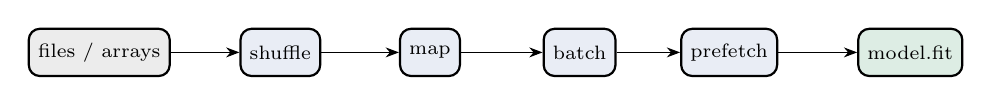
\begin{tikzpicture}[font=\scriptsize,b/.style={draw,thick,rounded corners,minimum height=0.6cm,fill=mlblue!10}]
\node[b,fill=gray!15] (a) at (0,0) {files / arrays};
\node[b] (b) at (2.3,0) {shuffle}; \node[b] (c) at (4.2,0) {map}; \node[b] (d) at (6.1,0) {batch}; \node[b] (e) at (8.0,0) {prefetch};
\node[b,fill=mlgreen!15] (f) at (10.3,0) {model.fit};
\draw[-Stealth] (a)--(b); \draw[-Stealth] (b)--(c); \draw[-Stealth] (c)--(d); \draw[-Stealth] (d)--(e); \draw[-Stealth] (e)--(f);
\end{tikzpicture}
\end{drawit}

\begin{numer}[: number of batches]
$n=1000$, batch size $32$: $\lceil1000/32\rceil=\lceil31.25\rceil=\mathbf{32}$ batches (31 full $+$ one of 8).\\ With \texttt{drop\_remainder=True}: $31$ batches.
\end{numer}

\subsection{The TFRecord format}
\begin{dfn}{TFRecord}
\textbf{TFRecord} is TensorFlow's preferred \textbf{binary} format for storing large data: a sequence of binary records, usually serialised \textbf{protocol buffers} (\texttt{tf.train.Example} with features of type bytes, float or int64). Read with \texttt{TFRecordDataset}; can be compressed (GZIP).
\end{dfn}
Advantages: fast to read, compact, supports any data (images, text), works well with \texttt{tf.data}.

\section{Preprocessing Data}
\textbf{Where to preprocess:} (1) beforehand (NumPy/Pandas), (2) in the \texttt{tf.data} pipeline with \texttt{map}, (3) with \textbf{Keras preprocessing layers} inside the model, so the same preprocessing is used in training and production (no \textbf{training/serving skew}).

\begin{center}
\small
\begin{tabular}{@{}p{4.6cm}p{11.7cm}@{}}
\toprule
\textbf{Layer} & \textbf{What it does}\\
\midrule
\texttt{Normalization} & standardise: $x'=(x-\mu)/\sigma$; $\mu,\sigma$ learned by \texttt{adapt()} on training data\\
\texttt{Discretization} & convert numbers into bins (categories)\\
\texttt{StringLookup}, \texttt{IntegerLookup} & map categories to integer indices (vocabulary, OOV buckets)\\
\texttt{CategoryEncoding} & one-hot / multi-hot encoding\\
\texttt{Hashing} & hash categories into a fixed number of bins\\
\texttt{Embedding} & dense trainable vector for each category (\#categories $\times$ dim parameters)\\
\texttt{TextVectorization} & split text into words and map to indices (or TF-IDF)\\
\texttt{Rescaling}, \texttt{Resizing}, \texttt{CenterCrop} & image preprocessing; \texttt{RandomFlip}, \texttt{RandomRotation} for augmentation\\
\bottomrule
\end{tabular}
\end{center}

\begin{dfn}{One-hot encoding vs.\ embedding}
\textbf{One-hot encoding} represents a category with $K$ categories as a vector of length $K$ with a single 1 (good for few categories). An \textbf{embedding} represents each category by a small \textbf{dense, trainable vector}; similar categories get similar vectors (good for many categories, e.g.\ words).
\end{dfn}
\begin{numer}[: preprocessing]
\textbf{Normalization} of $[2,4,6]$: $\mu=4$, $\sigma=\sqrt{8/3}=1.633$ $\Rightarrow$ $[-1.225,\,0,\,1.225]$.\\
\textbf{One-hot} with categories (red, green, blue): green $\to[0,1,0]$.\\
\textbf{Embedding} 50 categories, dimension 8: $50\times8=\mathbf{400}$ parameters.
\end{numer}
\begin{itemize}
  \item \textbf{TensorFlow Datasets (TFDS):} ready-made datasets (MNIST, IMDb, \dots) loaded with the function \texttt{tfds.load()}.
  \item \textbf{TF Transform:} preprocessing for production pipelines (TFX).
\end{itemize}
\apa{fast, scalable pipelines, GPU/TPU and distributed support, same preprocessing in training and deployment, production tools}{steeper learning curve than Keras alone, debugging graphs is harder, verbose low-level API}{training on huge image/text datasets, mobile and web deployment, recommendation systems, research}

\begin{imp}
Most asked: what is TensorFlow and its features; tensors and variables; \texttt{tf.data} methods and pipeline order; TFRecord; Keras preprocessing layers; one-hot vs.\ embedding.
\end{imp}

\begin{iq}
\item \twom What is a tensor? Give its rank examples.
\item \twom Differentiate \texttt{tf.constant} and \texttt{tf.Variable}.
\item \twom What is prefetching?
\item \twom What is a TFRecord file?
\item \fivem Explain automatic differentiation using \texttt{GradientTape}.
\item \fivem Explain the main methods of the \texttt{tf.data} API.
\item \fivem Compare one-hot encoding and embeddings.
\item \tenm Explain TensorFlow: architecture, tensors, operations and features.
\item \tenm Explain how data is loaded and preprocessed in TensorFlow using \texttt{tf.data}, TFRecord and Keras preprocessing layers.
\end{iq}

\backmatter
\chapter*{Last-Hour Revision Sheet}
\markboth{Last-Hour Revision Sheet}{}
\addcontentsline{toc}{chapter}{Last-Hour Revision Sheet}

\section*{1. Formulas you must know}
\begin{center}
\small
\renewcommand{\arraystretch}{1.45}
\begin{tabular}{@{}p{4.0cm}p{12.6cm}@{}}
\toprule
Least squares & $\theta_1=\frac{\sum(x-\bar x)(y-\bar y)}{\sum(x-\bar x)^2}$, $\ \theta_0=\bar y-\theta_1\bar x$, $\ R^2=1-\frac{\mathrm{SSE}}{\mathrm{SST}}$\\
Gradient descent & $\theta\leftarrow\theta-\alpha\,\partial J/\partial\theta$\\
Losses & MSE $\frac1n\sum(y-\hat y)^2$; MAE $\frac1n\sum|y-\hat y|$; log-loss $-[y\ln p+(1-y)\ln(1-p)]$\\
Bias--variance & $\E[(y-\hat f)^2]=\Bias^2+\Var+\sigma^2$\\
Metrics & Acc $\frac{TP+TN}{\text{all}}$, P $\frac{TP}{TP+FP}$, R $\frac{TP}{TP+FN}$, $F_1=\frac{2PR}{P+R}$\\
Standard error / CI & $\sigma/\sqrt n$; $\ \bar x\pm1.96\,s/\sqrt n$\\
Distances & Euclidean $\sqrt{\sum(a-b)^2}$, Manhattan $\sum|a-b|$, cosine $\frac{\vect a\cdot\vect b}{\|\vect a\|\|\vect b\|}$\\
Entropy / gain / Gini & $-\sum p\log_2p$; $\ H(S)-\sum\frac{|S_v|}{|S|}H(S_v)$; $\ 1-\sum p^2$\\
Bayes / Naive Bayes & $P(C|X)=\frac{P(X|C)P(C)}{P(X)}$; $\ \hat y=\argmax_cP(c)\prod P(x_j|c)$; Laplace $\frac{n+1}{N+V}$\\
Sigmoid / softmax & $\frac1{1+e^{-z}}$; $\ \frac{e^{z_k}}{\sum e^{z_j}}$; odds $\frac p{1-p}$\\
SVM & margin $\frac2{\|\vect w\|}$; soft margin $\frac12\|\vect w\|^2+C\sum\xi_i$; hinge $\max(0,1-yf)$\\
Kernels & poly $(\gamma\vect a\cdot\vect b+r)^d$; RBF $e^{-\gamma\|\vect a-\vect b\|^2}$; SVR $\max(0,|y-f|-\varepsilon)$\\
AdaBoost & $\alpha=\frac12\ln\frac{1-\varepsilon}{\varepsilon}$; $w_i\leftarrow w_ie^{-\alpha y_ih(\vect x_i)}$, normalise\\
OOB & $(1-1/n)^n\approx36.8\%$ left out\\
K-Means / silhouette & $J=\sum\|\vect x-\vect\mu\|^2$; $s=\frac{b-a}{\max(a,b)}$\\
GMM (E-step) & $\gamma_{ij}=\frac{\pi_j\mathcal N_j(\vect x_i)}{\sum_l\pi_l\mathcal N_l(\vect x_i)}$\\
PCA & $\mathbf C=\frac1{n-1}\tilde{\mathbf X}^{\!\top}\tilde{\mathbf X}$, $\mathbf C\vect w=\lambda\vect w$, explained $=\lambda_j/\sum\lambda$\\
Neuron / perceptron & $a=\varphi(\vect w\cdot\vect x+b)$; $w\leftarrow w+\eta(y-\hat y)x$\\
Dense layer parameters & $n_{\text{in}}n_{\text{out}}+n_{\text{out}}$\\
\bottomrule
\end{tabular}
\end{center}

\section*{2. Ten comparisons asked again and again}
\begin{center}
\small
\begin{tabular}{@{}p{4.2cm}p{5.8cm}p{5.8cm}@{}}
\toprule
\textbf{Pair} & \textbf{First} & \textbf{Second}\\
\midrule
Supervised / unsupervised & labelled data, predict $y$ & unlabelled, find structure\\
Batch / online & all data at once, retrain & incremental, streaming data\\
Instance / model-based & memorise + similarity (k-NN) & fit parameters (regression)\\
Underfit / overfit & high bias, too simple & high variance, too complex\\
Parameter / hyperparameter & learned from data (weights) & set before training ($k$, $C$, $\eta$)\\
Linear / logistic regression & number, MSE, closed form & probability, sigmoid, log-loss\\
Bagging / boosting & parallel, reduces variance & sequential, reduces bias\\
Hard / soft margin & no violations, outlier-sensitive & slack $\xi$, controlled by $C$\\
K-Means / DBSCAN & needs $k$, spherical & density, any shape, finds noise\\
Feature selection / extraction & subset of features & new features (PCA)\\
\bottomrule
\end{tabular}
\end{center}

\section*{3. Which algorithm? One line each}
\begin{center}
\small
\begin{tabular}{@{}p{3.4cm}p{13.2cm}@{}}
\toprule
k-NN & majority vote of $k$ nearest points; lazy; scale features\\
Decision tree & split on highest information gain (ID3) or Gini (CART); prune to avoid overfit\\
Naive Bayes & Bayes' theorem with independent features; smoothing; fast for text\\
Linear regression & least-squares line; $R^2$; normal equation or GD\\
Logistic regression & sigmoid of a linear score; log-loss; probability output\\
GLM & distribution $+$ linear predictor $+$ link (identity, logit, log)\\
SVM & widest street; support vectors; kernels for non-linear; $C$, $\gamma$\\
Random forest & bagged trees $+$ random features; vote\\
AdaBoost & reweight mistakes; weighted vote of stumps\\
Gradient boosting & each tree fits residuals; shrinkage $\eta$\\
Stacking & meta-learner combines base predictions\\
K-Means & assign to nearest centroid, update means; elbow/silhouette\\
DBSCAN & core (MinPts in $\varepsilon$), border, noise\\
GMM & mixture of Gaussians; EM; soft clusters\\
PCA & eigenvectors of covariance; keep 95\% variance\\
MLP & layers of neurons; backpropagation; ReLU, softmax\\
\bottomrule
\end{tabular}
\end{center}

\section*{4. Mock test (3 hours, 70 marks)}
\textbf{Section A} (answer all, $7\times2=14$)
\begin{enumerate}[label=\arabic*.]
  \item Define machine learning using $T$, $P$, $E$.
  \item What is the bias--variance trade-off?
  \item Define information gain.
  \item What are support vectors?
  \item What is out-of-bag evaluation?
  \item What is the curse of dimensionality?
  \item Why are activation functions needed in an MLP?
\end{enumerate}
\textbf{Section B} (any four, $4\times7=28$)
\begin{enumerate}[label=\arabic*.,resume]
  \item Explain types of ML systems with examples.
  \item Explain k-fold cross-validation and compute $\mathrm{CV}_{(5)}$ for fold errors $0.10,0.12,0.08,0.11,0.09$. \emph{(Ans.\ 0.10)}
  \item Find the k-NN prediction ($k=3$) for $(5,4)$ using the data of Chapter~\ref{n:knn}.
  \item Compare bagging and boosting.
  \item Explain DBSCAN with core, border and noise points.
  \item Explain the \texttt{tf.data} pipeline.
\end{enumerate}
\textbf{Section C} (any two, $2\times14=28$)
\begin{enumerate}[label=\arabic*.,resume]
  \item Fit $\hat y=\theta_0+\theta_1x$ to $x=(1,2,3,4,5)$, $y=(35,45,50,65,70)$; predict $x=6$; compute $R^2$. \emph{(Ans.\ $26+9x$, 80, 0.976)}
  \item Explain SVM classification (linear and kernel) and SVR.
  \item Apply PCA to $(1,1),(2,3),(3,2),(4,5),(5,4)$ and find the explained variance of PC1. \emph{(Ans.\ 90\%)}
  \item Explain the MLP, backpropagation and the Keras workflow.
\end{enumerate}

\begin{imp}
Night before the exam: read only the definition boxes, this sheet and the important questions. In the exam: definition first, diagram second, points third, numerical/example fourth, advantages--disadvantages--applications last.
\end{imp}

\end{document}
